\documentclass[10pt]{article}
\usepackage{comment}
\usepackage[utf8]{inputenc}
\usepackage[T1]{fontenc}
\usepackage{amsmath,amsfonts,amssymb}
\usepackage{graphicx}
\usepackage{caption}
\usepackage{subcaption}
\usepackage{hyperref}
\usepackage{geometry}
\usepackage{fancyhdr}
\usepackage{float}
\usepackage{cite}
\usepackage{listings}
\usepackage{xcolor}
\usepackage{authblk}
\geometry{margin=0.75in}

\title{\textbf{Anomaly Detection with QML: A Benchmark study using different approaches with Pennylane}}

\author[1]{Jacopo Martellotto}
\affil[1]{\small\texttt{j.martellotto@studenti.unipi.it}}
\date{}

\author[2]{Federico Morano}
\affil[2]{\small\texttt{f.morano1@studenti.unipi.it}}
\date{} 

\pagestyle{fancy}
\fancyhf{}
\rhead{\thepage}
\lhead{Quantum Machine Learning Report}

\begin{document}

\maketitle

\section{Introduction}
The exponential growth of digital transactions and the increasing sophistication of cyber threats have made fraud detection a critical and challenging task. Traditional machine learning methods have shown promising results in identifying anomalies within large-scale datasets; however, their limitations in scalability, privacy, and computational cost highlight the need for exploring more advanced paradigms.\\
This project investigates the use of QML techniques to enhance fraud detection systems, with a particular focus on identifying the most accurate and efficient approaches. Our research compares and evaluates several architectures and strategies, including Quantum Neural Networks (QNNs), Quantum Federated Learning (QFL), and a selection of classical machine learning algorithms commonly used for anomaly detection.\\
In all QML-based experiments, we employ hybrid models that combine classical and quantum layers, leveraging the representational power of quantum circuits while retaining the stability and scalability of classical neural networks.\\
For the federated learning scenario, our architecture emphasizes data privacy and security. Instead of sharing raw data, each client trains its model locally and only transmits encrypted model parameters to the aggregator. To enforce privacy and trust in this decentralized setting, we integrate blockchain technology for verifiable model sharing and quantum cryptography techniques such as simulated Quantum Key Distribution (QKD) and homomorphic encryption. This ensures secure and tamper-resistant communication between clients and the central server without compromising sensitive data.\\
By systematically comparing these approaches across a benchmarked fraud detection task, the goal of this project is to determine which paradigm—classical, quantum, or hybrid—offers the best trade-off between accuracy, privacy, and computational efficiency in anomaly detection.

\section{About Dataset}
For our experiments, we utilize the Credit Card Fraud Detection dataset, which is publicly available on Kaggle. It contains 20k+ transactions and it's highly imbalanced. The dataset is made up of 114 columuns. Obviously, the last one \texttt{targets} is the target column, which indicates whether a transaction is fraudulent (1) or not (0). The dataset has been preprocessed to remove any personally identifiable information, ensuring that it can be used for research purposes without compromising privacy.\\
Before Preprocessing, let's analyze the dataset. In order to evaluate how features are correlated each other, we can use the correlation matrix. The correlation matrix is a table that shows the correlation coefficients between many variables. Each cell in the table displays the correlation between two variables. The values range from -1 to 1. The heatmap of the correlation matrix can help us visualize these relationships more clearly. In the figure below, we present the correlation heatmap of the most relevant 30 features. 
\begin{figure}[h!]
	\centering
	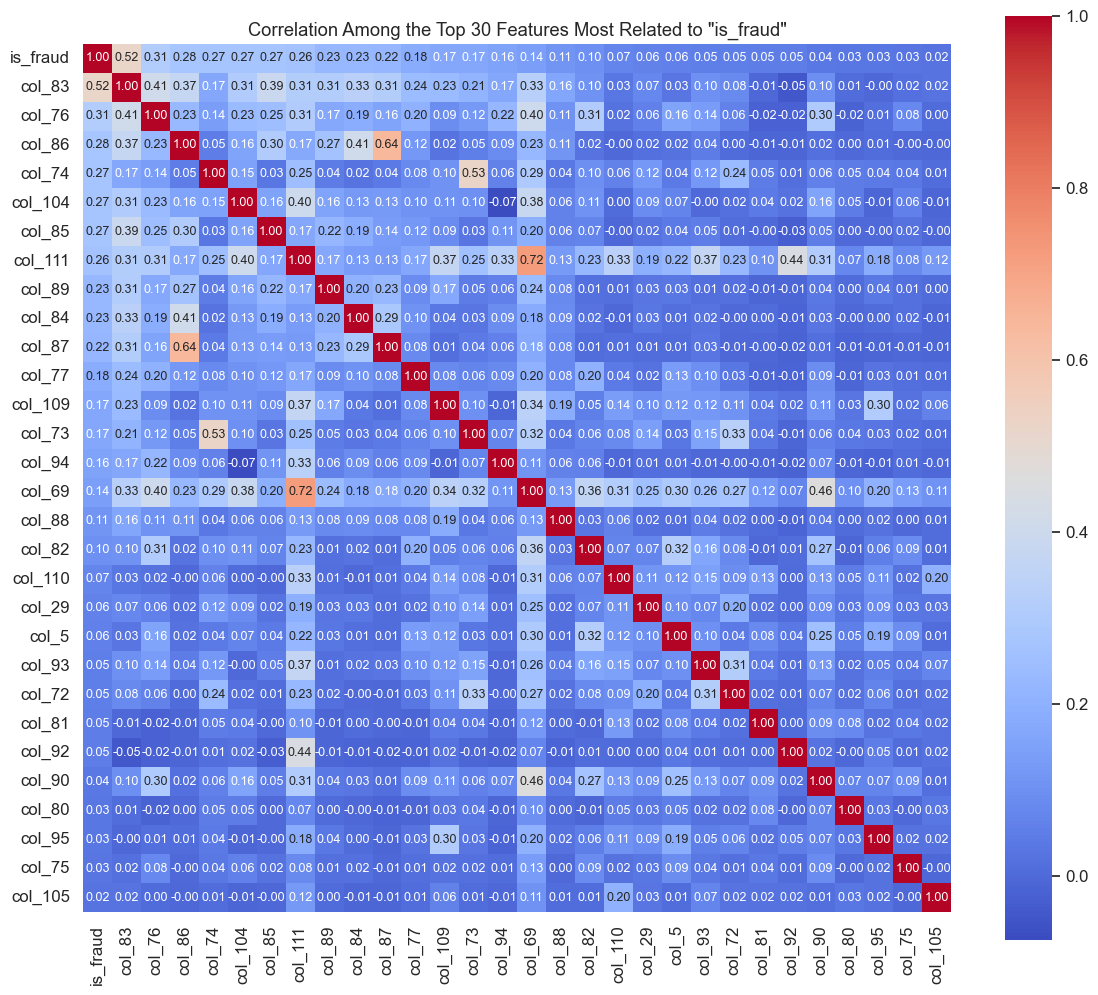
\includegraphics[height = 0.6\textheight]{img/correlation_heatmap_top_30_features.png}
	\caption{Correlation heatmap of the top 30 features in the Credit Card Fraud Detection dataset. Darker colors indicate stronger correlations between features, while lighter colors indicate weaker correlations. This visualization helps identify potential relationships and interactions between variables that may be relevant for fraud detection.}
\end{figure}


\section{Preprocessing}
An essential step in the development of a predictive model is data preprocessing, which includes all the necessary operations to make the dataset suitable for analysis. In our case, the dataset is significantly imbalanced: fraudulent transactions represent only a small fraction compared to legitimate ones. This class imbalance can severely affect the performance of classification models, leading them to favor the majority class and, as a result, reducing their ability to correctly detect fraud, which is the primary focus of the analysis.\\
To address this issue, we explored two common approaches: undersampling of the majority class and oversampling of the minority class.
\begin{itemize}
    \item \textit{Undersampling} reduces the number of samples in the majority class (i.e., legitimate transactions) by randomly selecting a subset. While this method can quickly balance the dataset, it risks discarding valuable information, potentially decreasing the model’s generalization capabilities.
    \item \textit{Oversampling} increases the number of minority class samples. In particular, we adopted the SMOTE (Synthetic Minority Oversampling Technique) method, which generates synthetic samples instead of duplicating existing ones. This helps to enrich the distribution of the minority class in feature space.
\end{itemize}
\subsubsection*{SMOTE: Synthetic Minority Oversampling Technique}
SMOTE works by creating new synthetic examples of the minority class in feature space. Given a sample \( \mathbf{x}_i \) from the minority class, the algorithm selects its \( k \)-nearest neighbors (typically \( k = 5 \)). One of these neighbors, \( \mathbf{x}_{zi} \), is chosen at random. A new synthetic sample \( \mathbf{x}_{\text{new}} \) is then generated as a convex combination of \( \mathbf{x}_i \) and \( \mathbf{x}_{zi} \), using the formula:
\[
\mathbf{x}_{\text{new}} = \mathbf{x}_i + \lambda \cdot (\mathbf{x}_{zi} - \mathbf{x}_i)
\]
where \( \lambda \in [0, 1] \) is a random number. This process effectively expands the decision region of the minority class, producing samples that lie along the lines connecting existing samples and their neighbors, thus helping the classifier learn more generalized boundaries.
\subsubsection*{Comparison and Method Selection}
We tested both approaches in a separate workspace (not included in the main project directory) by training a standard Random Forest classifier on each preprocessed dataset. The performance of the models was then evaluated using standard classification metrics, including accuracy, precision, recall, and F1-score.
The results indicated that the dataset generated using SMOTE significantly outperformed the one obtained through undersampling, especially in terms of recall for the minority class. This improvement demonstrates SMOTE’s effectiveness in addressing class imbalance without sacrificing overall model performance. Consequently, SMOTE was selected as the official resampling strategy for the data preprocessing pipeline.
\begin{figure}[h!]
	\centering
	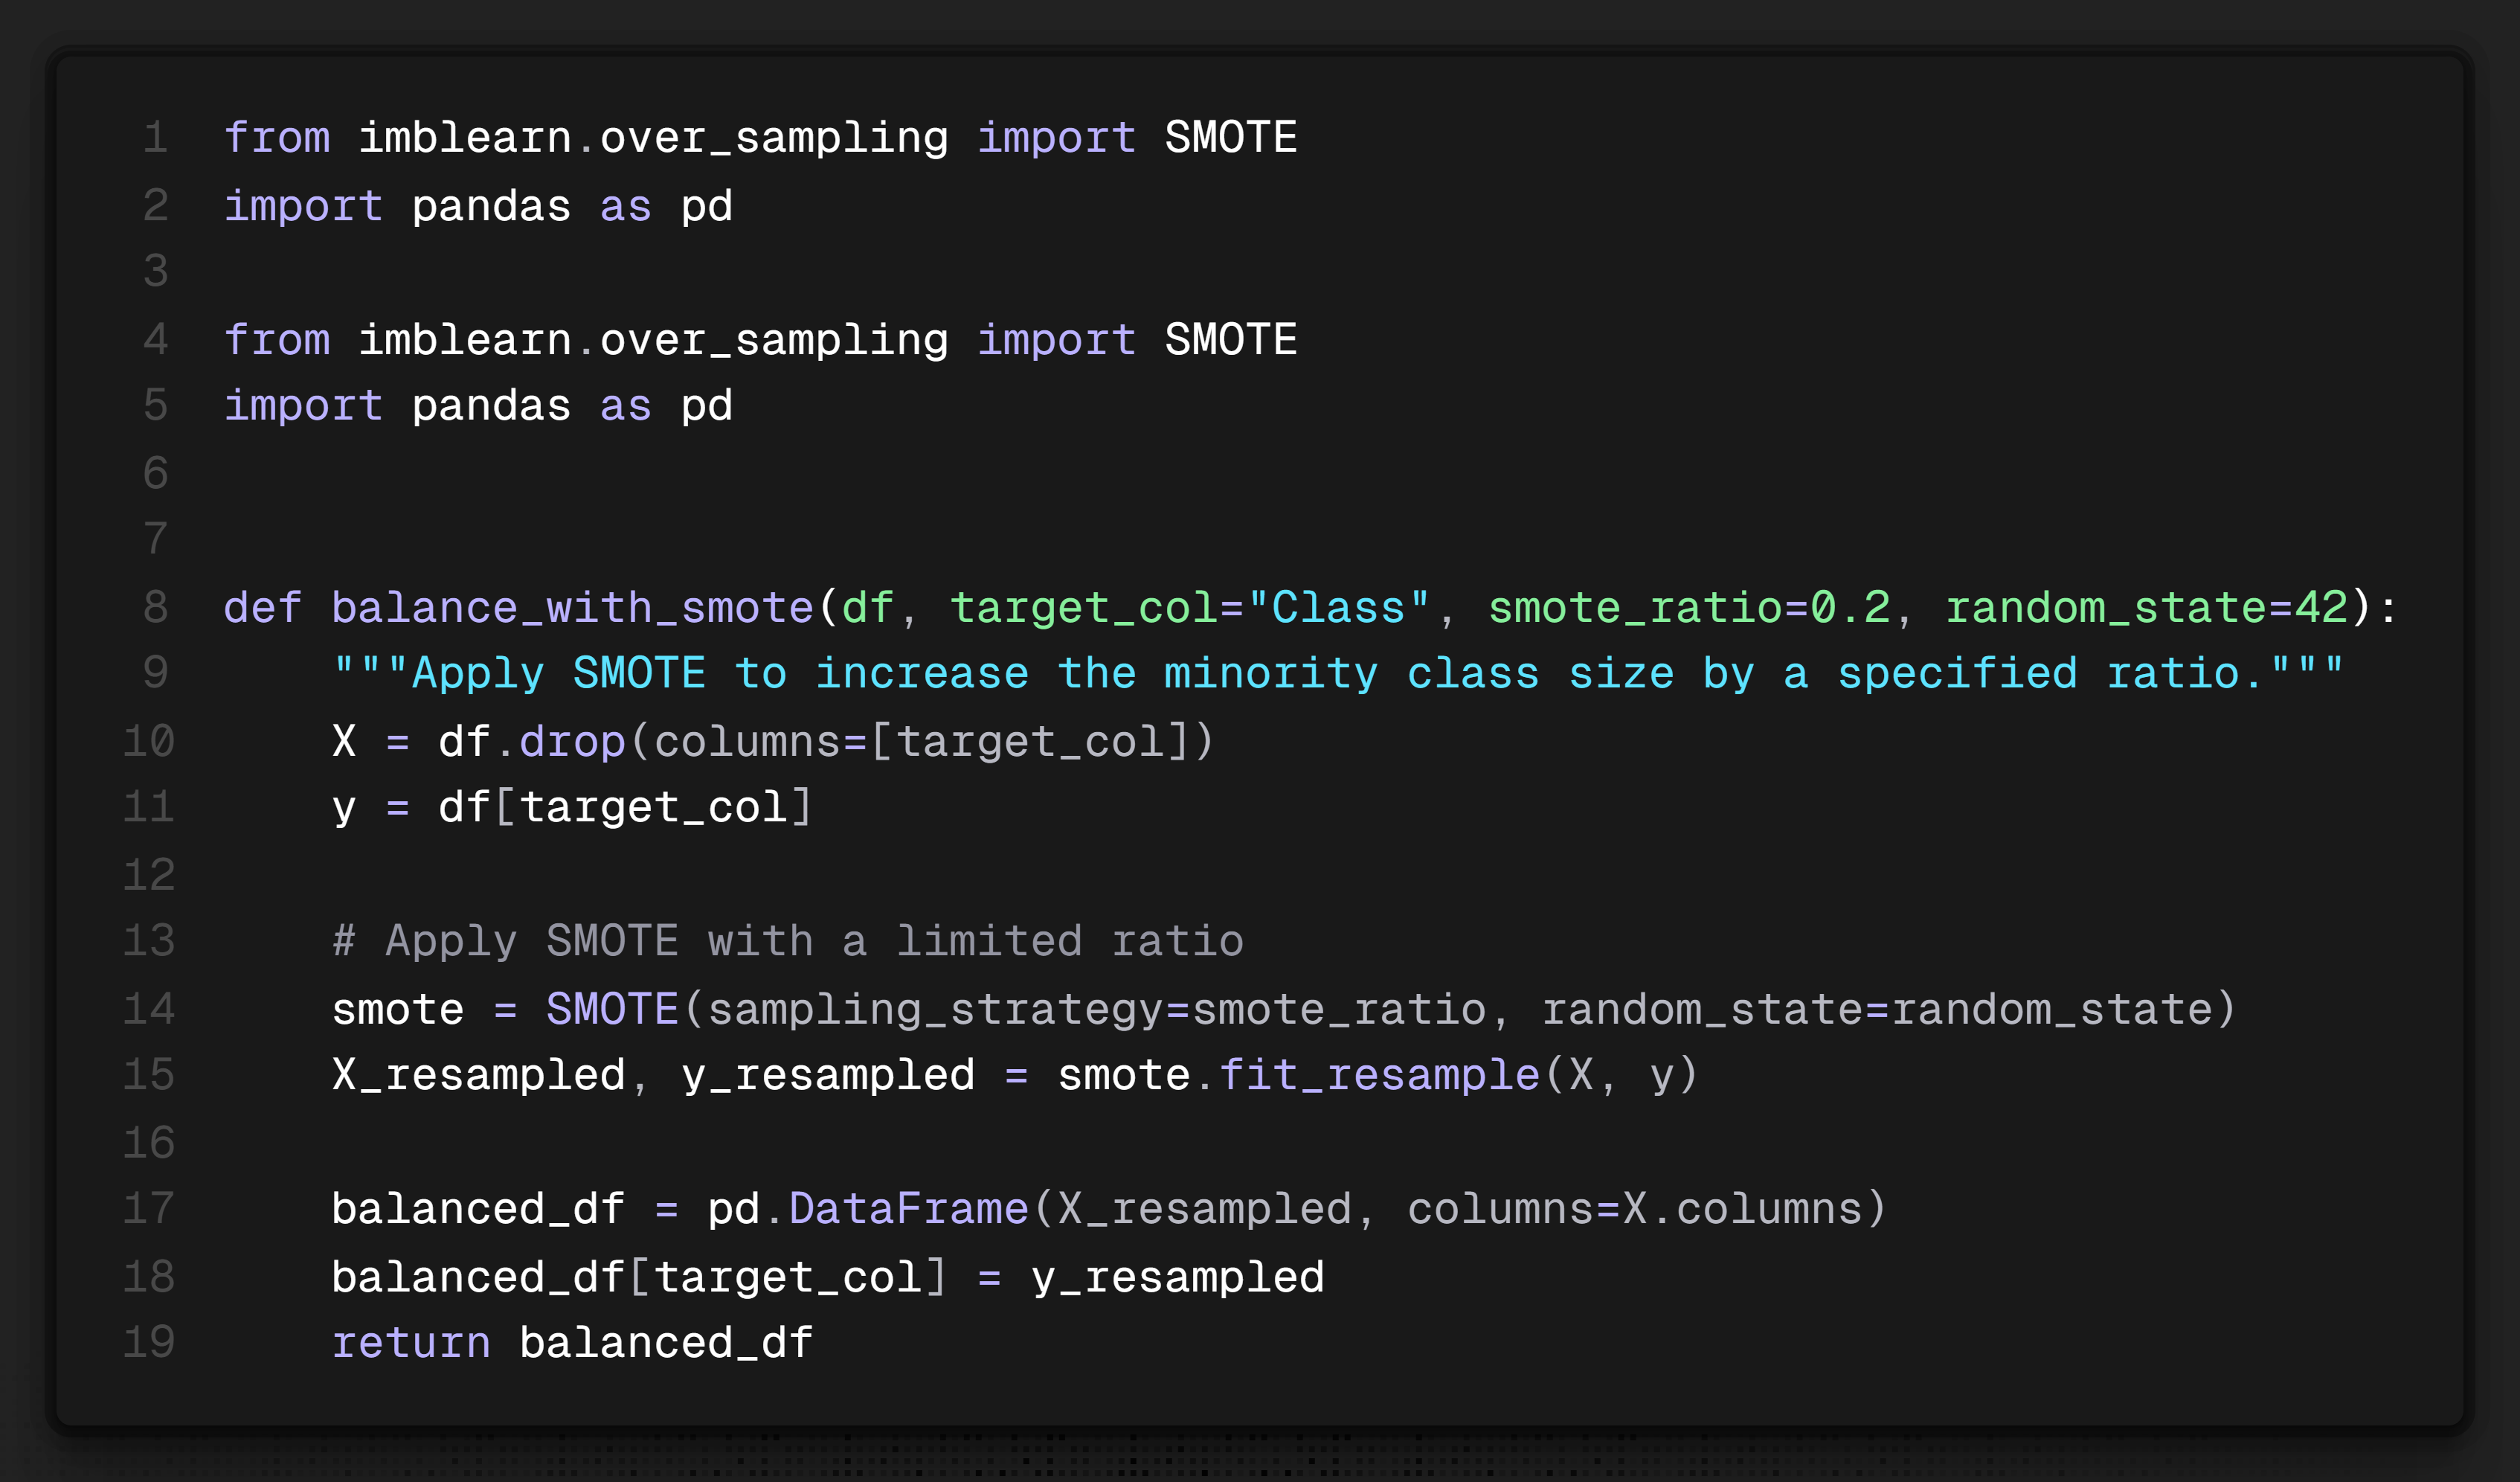
\includegraphics[height = 0.30\textheight]{img/SMOTE.png}
	\caption{Implementation of the SMOTE algorithm in Python.}
\end{figure}

\section{Classic Machine Learning}
In order to benchmark the performance of quantum machine learning models, we first implemented a series of classical machine learning algorithms. These algorithms serve as a baseline for comparison with quantum-enhanced approaches. The following classical models were trained and evaluated on the preprocessed dataset:
\begin{itemize}
	\item \textbf{Dummy}
	\item \textbf{Decision Tree (DT)}
	\item \textbf{AdaBoost}
	\item \textbf{Multi-Layer Perceptron (MLP)}
	\item \textbf{Logistic Regression (LR)}
	\item \textbf{Random Forest (RF)}
	\item \textbf{Support Vector Machine (SVM)}
	\item \textbf{K-Nearest Neighbors (KNN)}
\end{itemize}
We expect that RF may be the most effective classical model for our dataset, given its ability to handle imbalanced data and capture complex interactions between features. In the following lines, we present our comparing results, which include the accuracy, precision, recall, and F1-score for each model. These metrics provide a comprehensive evaluation of the models' performance in detecting fraudulent transactions.
\begin{figure}[H]
	\centering
	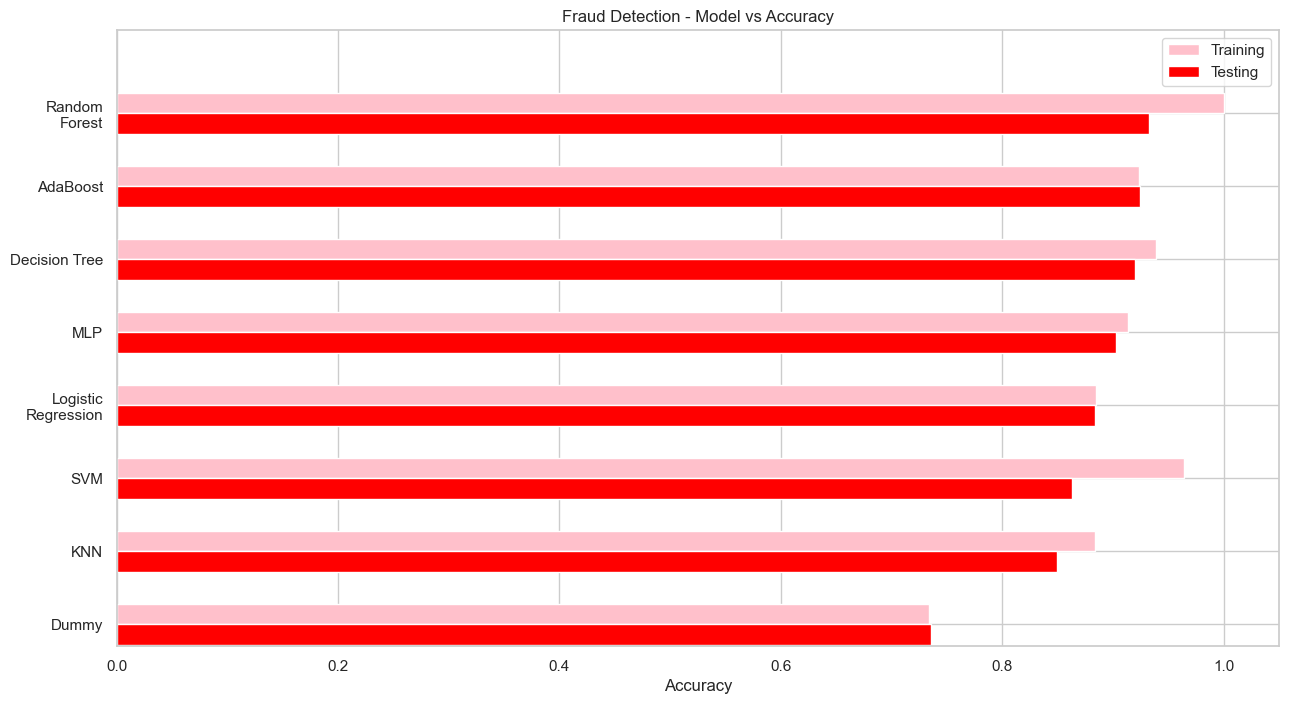
\includegraphics[height = 0.40\textheight]{img/fraud_detection_model_accuracy.png}
	\caption{Model vs Accuracy - Random Forest (RF) achieved the highest accuracy, as expected.}
\end{figure}
\begin{figure}[H]
	\centering
	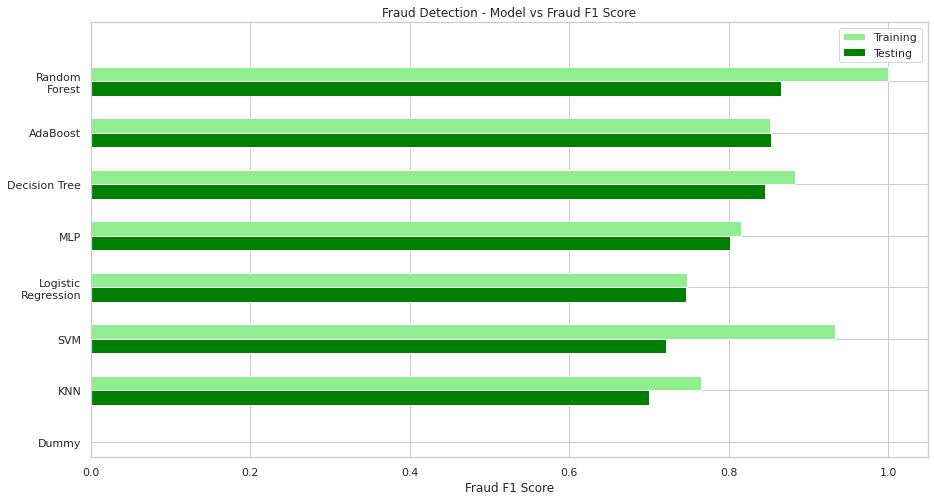
\includegraphics[height = 0.40\textheight]{img/fraud_f1_score.png}
	\caption{Model vs F1-Score - Random Forest achieved the highest F1-Score, indicating a good balance between precision and recall.}
\end{figure}
\begin{figure}[H]
	\centering
	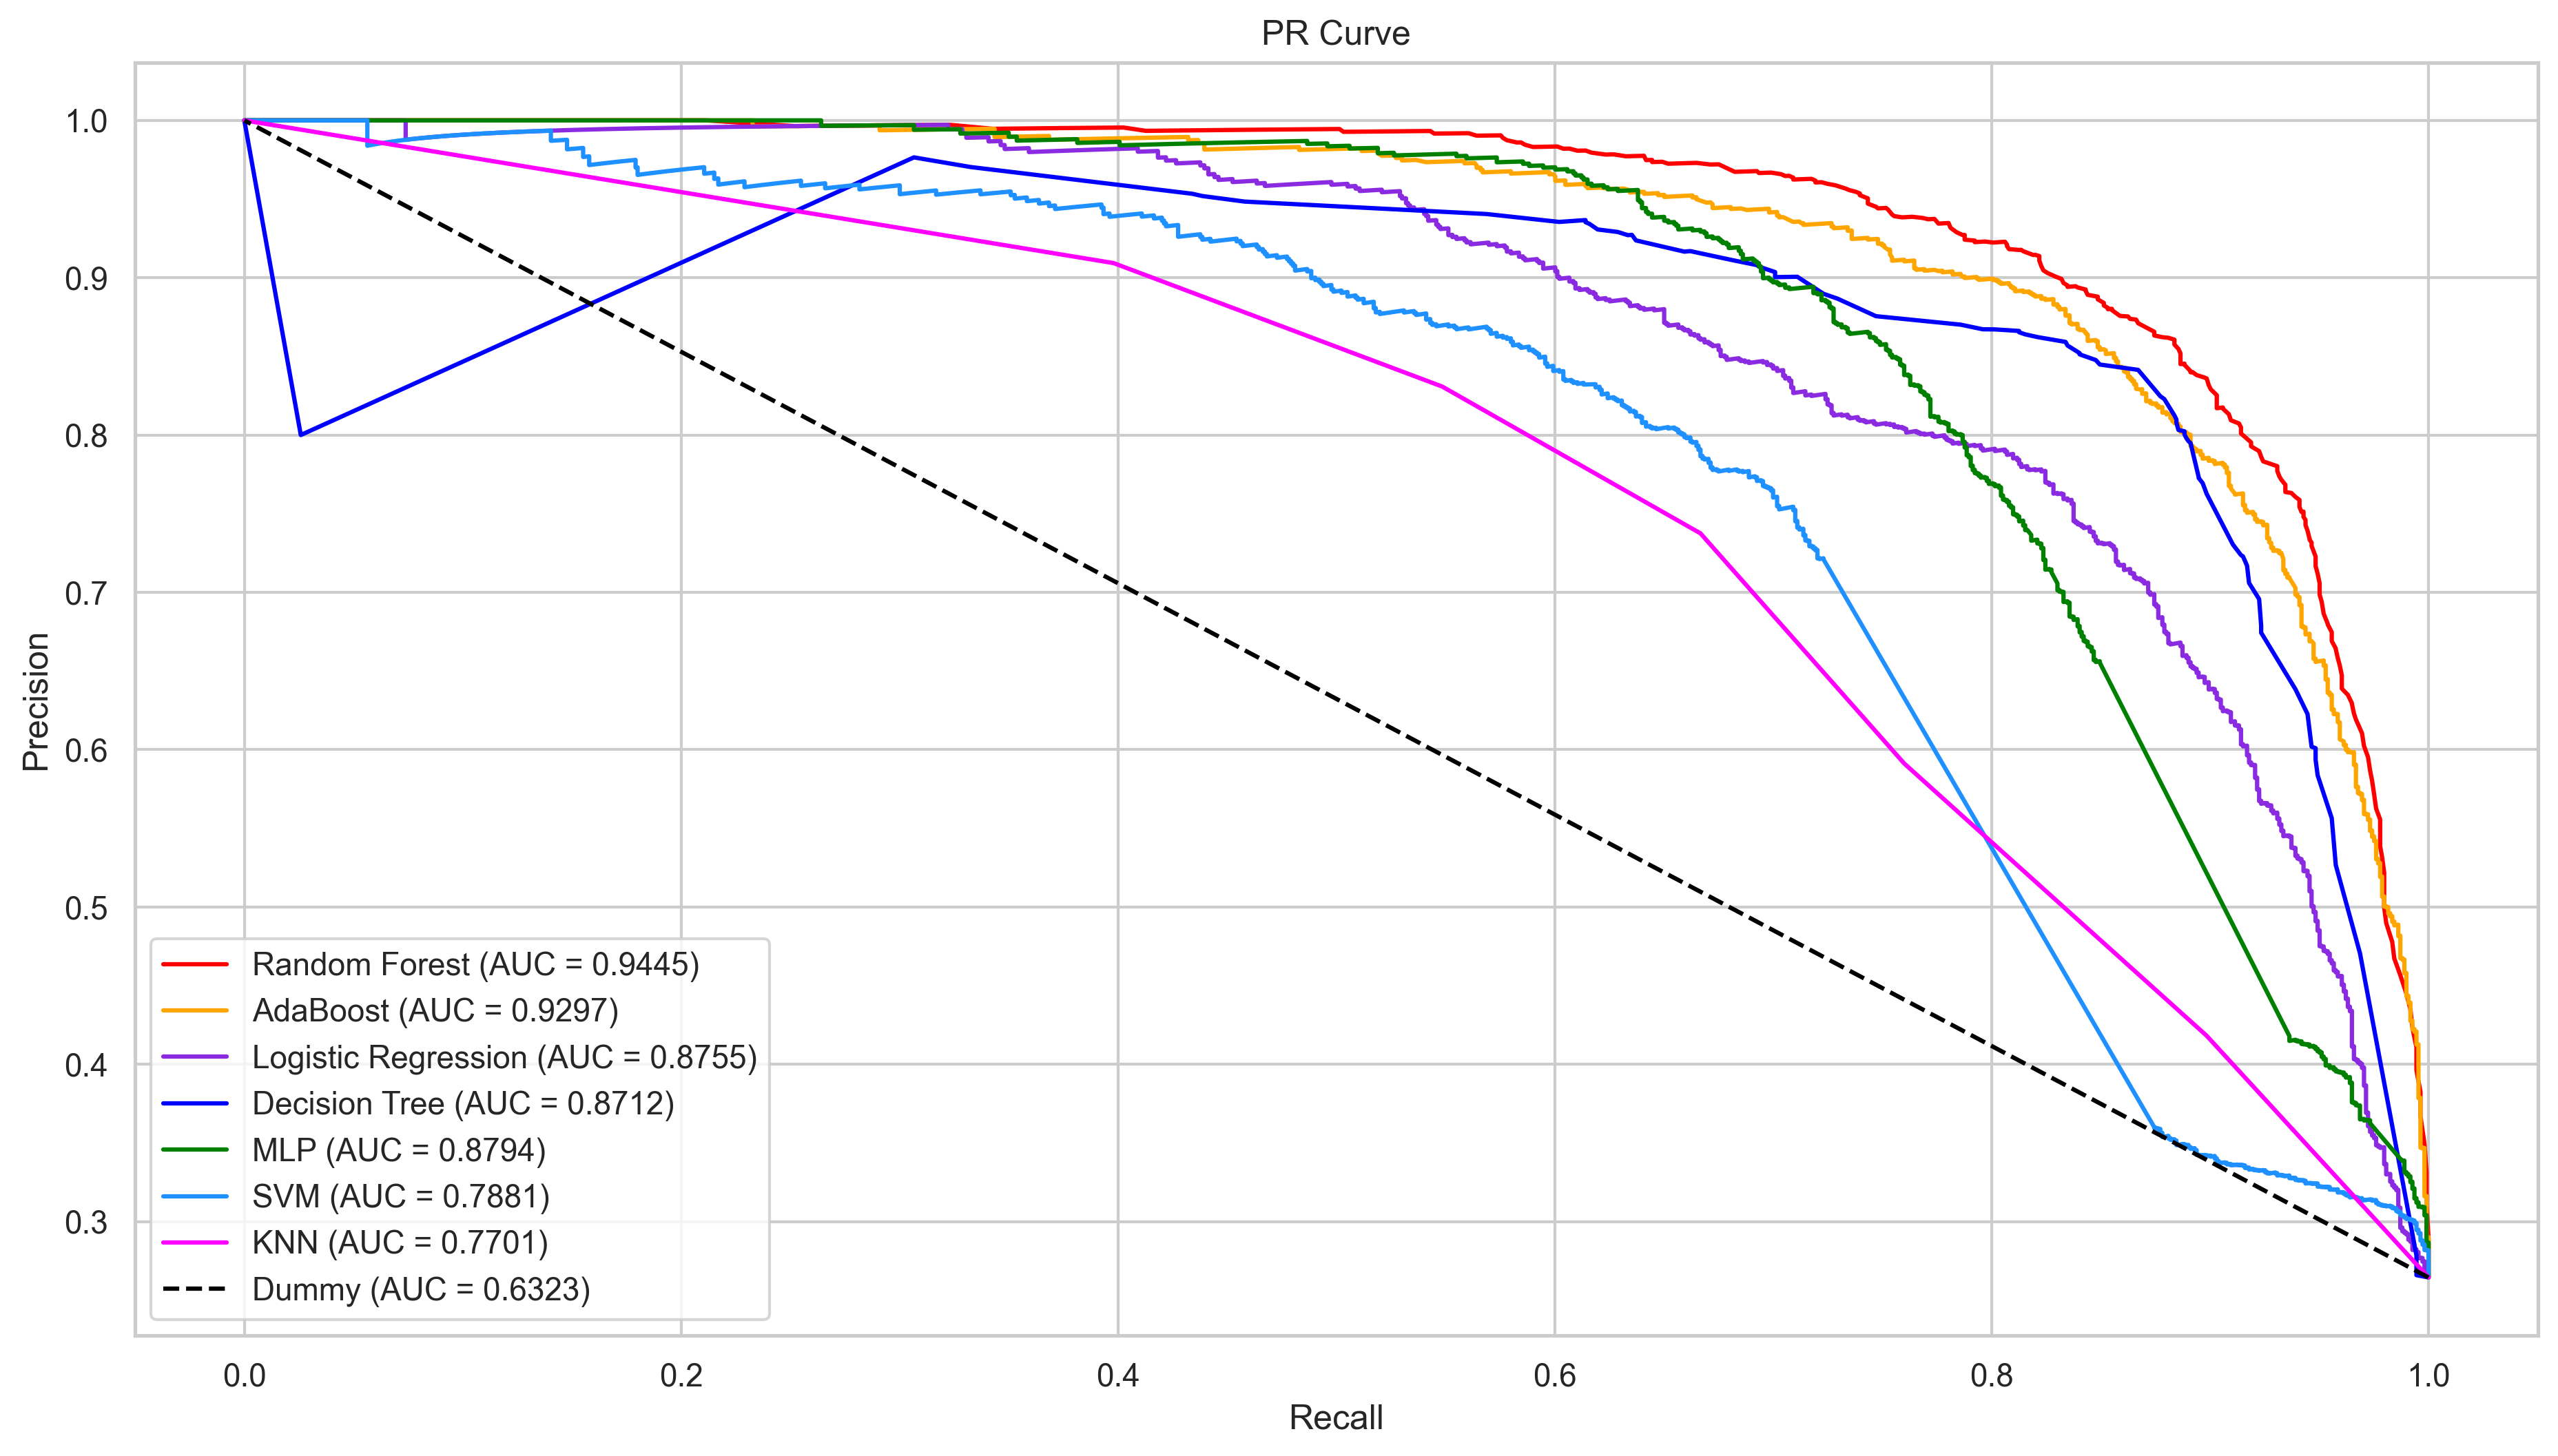
\includegraphics[height = 0.40\textheight]{img/PR_Curve.png}
	\caption{PR-Curve}
\end{figure}
\begin{figure}[H]
	\centering
	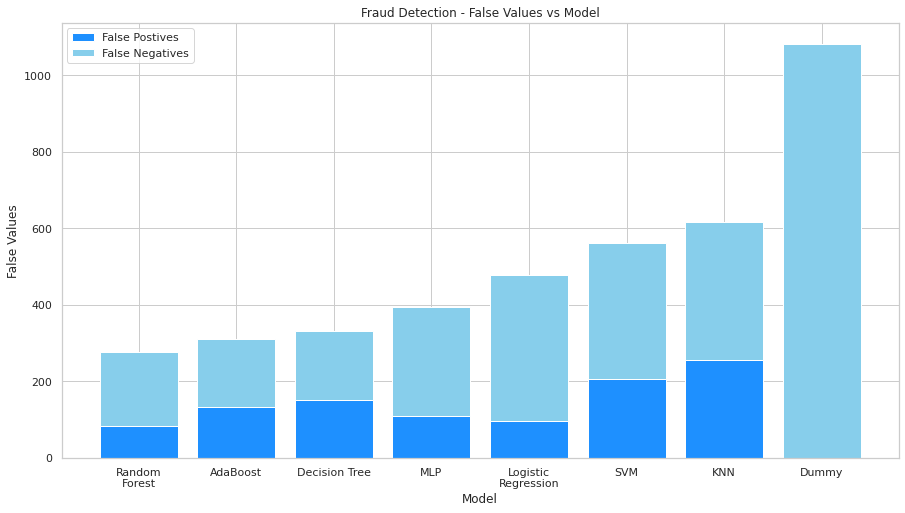
\includegraphics[height = 0.40\textheight]{img/fraud_detection_false_values.png}
	\caption{False Values - The chart shows the number of false positives and false negatives for each model.}
\end{figure}
We obtain the following results for each classical model:
\begin{table}[H]
	\centering
	\begin{tabular}{|l|c|c|c|c|c|}
		\hline
		Model & $\alpha$ optimized for & Accuracy (\%) & Precision (\%) & Recall (\%) & F1-Score (\%) \\
		\hline
		Dummy & – & 73.6 & 54.1 & 73.5 & 62.3 \\
		\hline
		Decision Tree & Accuracy & 91.4 & 91.3 & 91.4 & 91.3 \\
		Decision Tree & F1-Score & 91.9 & 91.9 & 91.9 & 91.9 \\
		\hline
		AdaBoost & Accuracy & 92.2 & 92.1 & 92.2 & 92.1 \\
		AdaBoost & F1-Score & 92.4 & 92.3 & 92.4 & 92.4 \\
		\hline
		MLP & Accuracy & 89.9 & 89.7 & 89.9 & 89.5 \\
		MLP & F1-Score & 90.3 & 90.2 & 90.3 & 89.9 \\
		\hline
		Logistic Regression & Accuracy & 88.2 & 88.2 & 88.2 & 87.6 \\
		Logistic Regression & F1-Score & 88.4 & 88.4 & 88.4 & 87.8 \\
		\hline
		Random Forest & Accuracy & 93.0 & 92.9 & 93.0 & 92.9 \\
		Random Forest & F1-Score & 93.2 & 93.2 & 93.2 & 93.1 \\
		\hline
		SVM & Accuracy & 86.2 & 85.8 & 86.2 & 85.6 \\
		SVM & F1-Score & 86.3 & 85.9 & 86.3 & 85.9 \\
		\hline
		KNN & Accuracy & 85.1 & 84.6 & 85.2 & 84.6 \\
		KNN & F1-Score & 84.9 & 85.5 & 84.9 & 84.6 \\
		\hline
	\end{tabular}
	\caption{Performance metrics for each model with hyperparameter $\alpha$ optimized separately for Accuracy and F1-Score.}
\end{table}
\noindent From the analysis of the results, we can draw the following conclusion: Randoma Forest performed the best overall, achieving the highest accuracy and F1-score. This is consistent with our expectations, as RF is known for its robustness in handling imbalanced datasets and capturing complex feature interactions. The Decision Tree and AdaBoost models also performed well, particularly when optimizing for F1-score. However, they did not surpass the performance of Random Forest. The other models, while still effective, showed lower performance metrics compared to RF, indicating that they may not be as suitable for this specific fraud detection task.\\
However, AdaBoost and Decision Tree models are also great choices for fraud detection since they have less false-negatives than Random Forest, which is a crucial aspect in fraud detection, where missing a fraudulent transaction can have significant consequences.\\


\section{Quantum Machine Learning}
\subsection{QNN}




\subsection{QFNN}
\begin{figure}[h!]
	\centering
	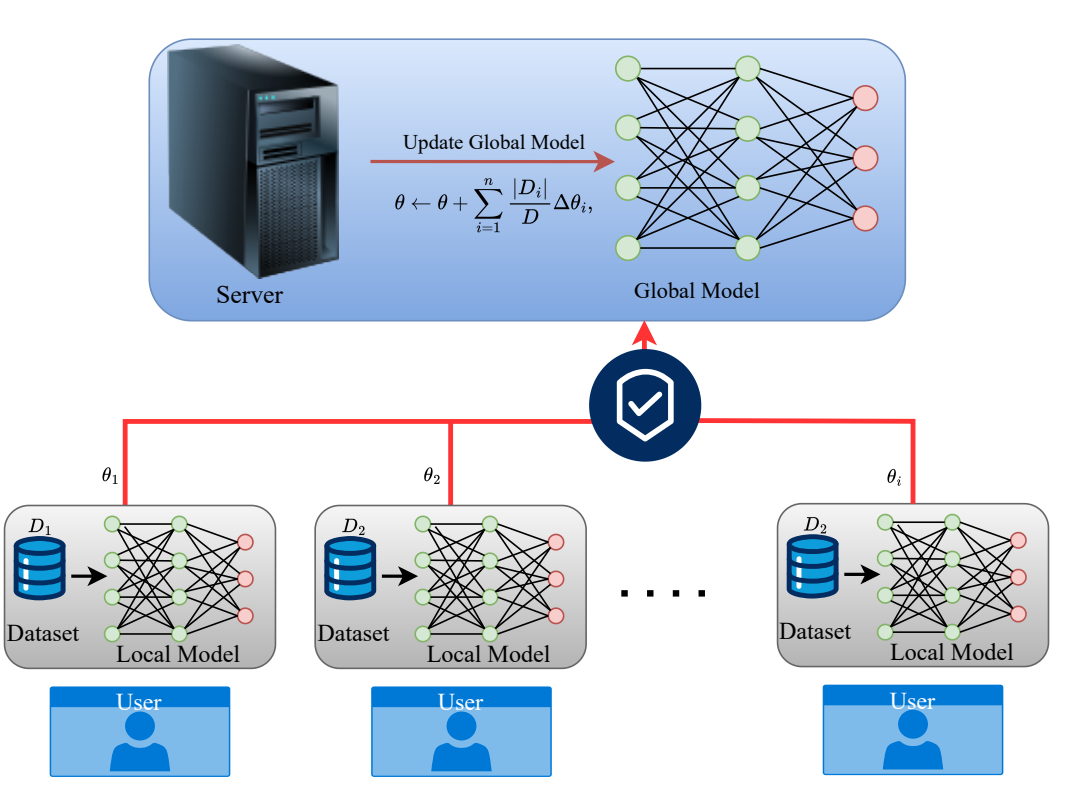
\includegraphics[height = 0.30\textheight]{img/FL_model.png}
	\caption{A schematic overview of the Federated Learning (FL) architecture illustrates several users (clients), each working with their own private dataset to independently train local models. Instead of sharing raw data, clients send their model updates to a central server. The server combines these updates to enhance the global model, which is then redistributed to all clients for the next training round. This iterative process preserves data privacy and security by ensuring that users' raw data remains on their local devices.}
\end{figure}
Federated Learning (FL) has recently gained prominence due to growing concerns about data privacy and the limitations of cloud-based deep learning with large-scale datasets. This learning paradigm involves two main components: a central server and multiple client nodes. The central server maintains the global model and collects the locally trained parameters from client devices. It then aggregates these parameters to update the global model, which is subsequently shared back with all clients. Each client trains the received model using its own local data, which typically represents only a small subset of the overall dataset.
In our proposed framework, the client nodes consist of quantum computers or quantum simulators that train circuit parameters using a hybrid quantum-classical approach. During each training round, a selected group of client nodes carries out local training. Afterward, the updated circuit parameters from all participating clients are sent to the central node, where they are aggregated to refine the global model.
\begin{figure}[h!]
	\centering
	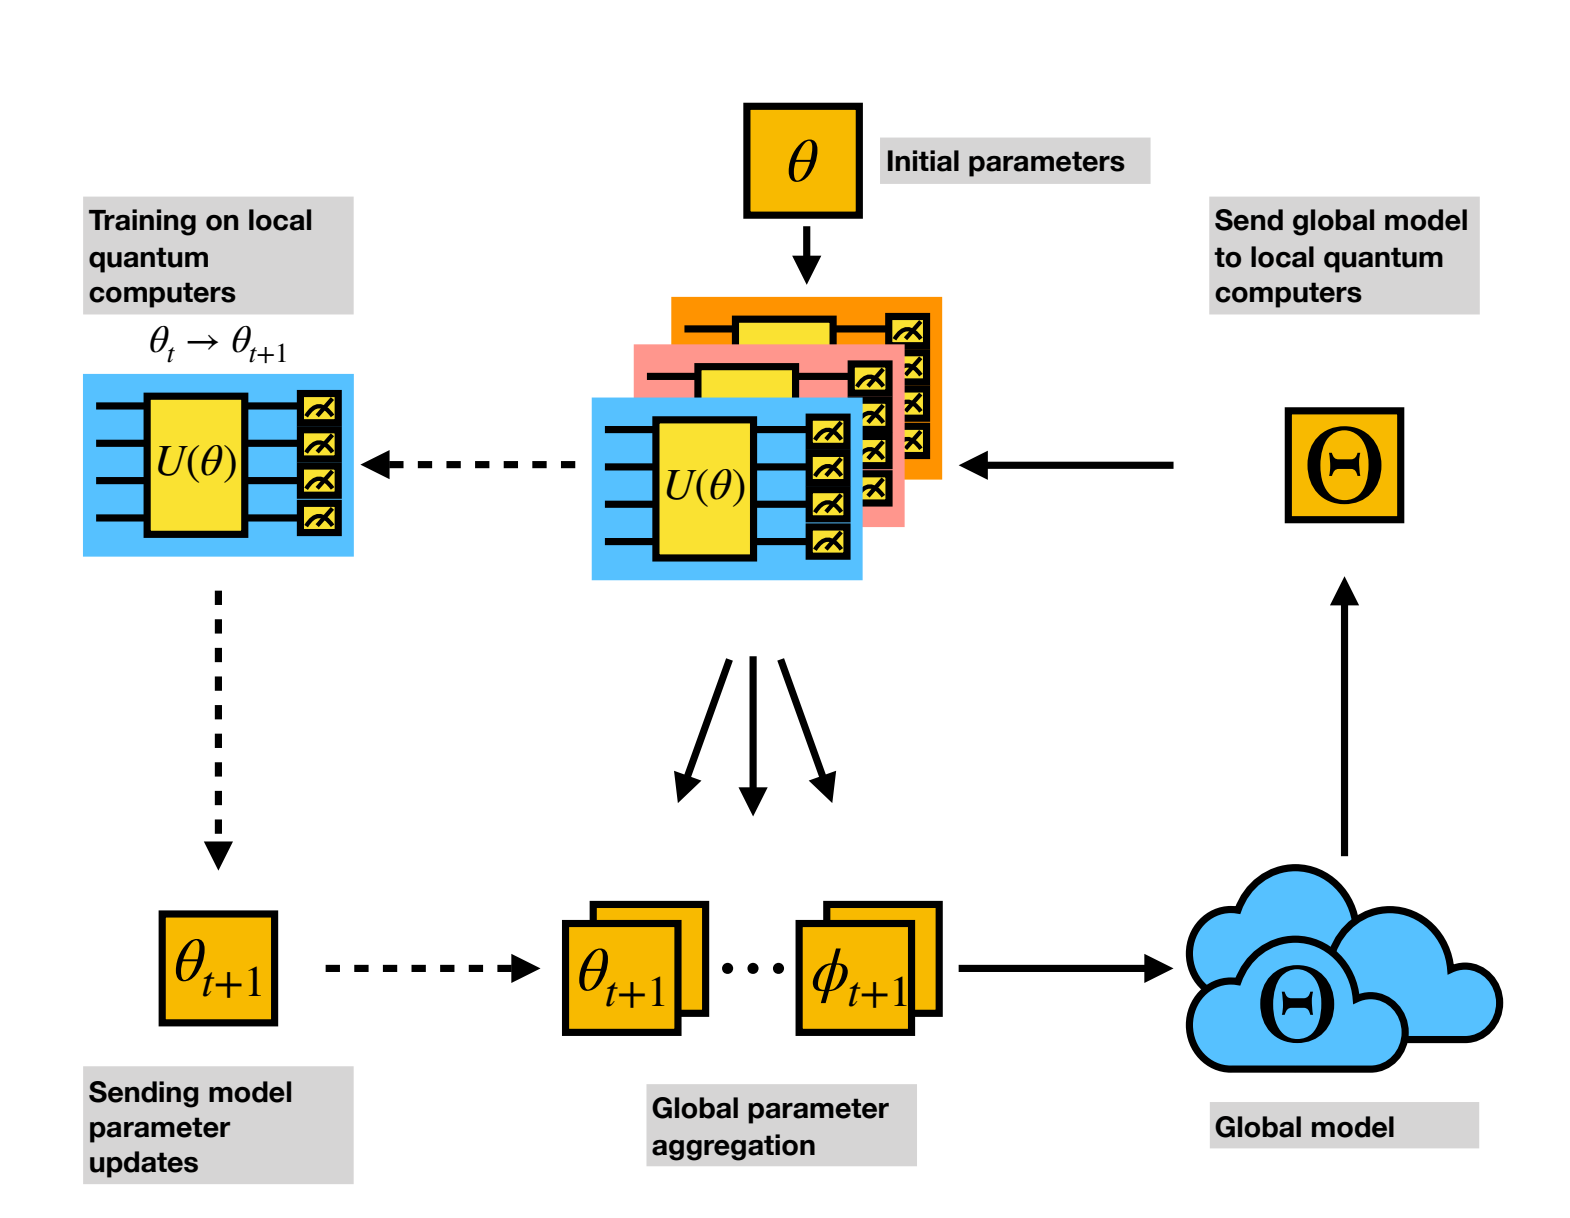
\includegraphics[height = 0.30\textheight]{img/QFL.png}
	\caption{Federated Quantum Learning (QFL)}
\end{figure}
The proposed solution emphasizes both privacy preservation and improved model performance by combining the computational power of quantum-enhanced models with the collaborative nature of federated learning.\\
This solution enables decentralized model training while ensuring that sensitive financial data remains private and secure. The system incorporates several advanced components, including quantum machine learning, homomorphic encryption, blockchain for model integrity, and a dynamic client-weighting mechanism for adaptive learning.
Let's analyze the architecture and key features of this project in detail:
\begin{itemize}
	\item \textbf{Quantum Federated Learning (QFL)}: Integrates quantum computing techniques within a federated learning framework to enhance model training at client nodes using quantum neural networks (QNNs).
	\item \textbf{Privacy Preservation}: Sensitive data remains on local devices and is never shared directly. Security is ensured using homomorphic encryption, quantum key distribution (QKD), and secret sharing protocols, preventing unauthorized access to model updates.
	\item \textbf{Adaptive Federated Learning}: The contribution of each client to the global model is dynamically adjusted based on local performance. Clients with higher accuracy have a greater influence on the aggregation process, thereby improving overall model robustness.
	\item \textbf{Homomorphic Encryption}: Model updates are encrypted during transmission using homomorphic encryption, which allows arithmetic operations to be performed directly on encrypted data without decryption, ensuring confidentiality throughout the training process.
	\item \textbf{Blockchain Integration}: Blockchain (Ethereum) is used to store hashed versions of the aggregated model weights, ensuring transparency, auditability, and protection against tampering through an immutable and decentralized ledger.
\end{itemize}
The implementation of the project relies on a combination of quantum computing libraries, machine learning frameworks, cryptographic techniques, and blockchain technologies:
\begin{itemize}
	\item \textbf{PennyLane}
	\item \textbf{TensorFlow/Keras}
	\item \textbf{TenSEAL}
	\item \textbf{Shamir's Secret Sharing}
	\item \textbf{Ethereum (via Web3)}: A smart contract is deployed to a local Ethereum test network (simulated using Ganache) to store and verify the integrity of model updates in a tamper-proof, decentralized manner.
	\item \textbf{Quantum Key Distribution (QKD)}: Simulated QKD is used for secure key exchange between clients, allowing encrypted communication channels for transmitting model updates securely across the network.
	\item \textbf{SMOTE (Synthetic Minority Oversampling Technique)}
\end{itemize}


\subsubsection{Adaptive Federated Learning Workflow}
The federated learning process is executed in multiple rounds and consists of the following key stages:
\begin{enumerate}
	\item \textbf{Local Training}: Each client trains a hybrid quantum-classical model locally using their own dataset. The data remains on the client’s device and is never shared externally. The resulting model updates are encrypted using homomorphic encryption.
	\item \textbf{Adaptive Client Selection}: Clients are evaluated based on their local performance on a validation set. Only clients exceeding a predefined accuracy threshold are selected to contribute to the global model, ensuring high-quality updates.
	\item \textbf{Weighted Aggregation}: Selected clients send their encrypted updates, which are then aggregated using a performance-weighted average. This process gives more influence to models that demonstrate higher accuracy, thereby enhancing the overall performance of the global model.
	\item \textbf{Secure Communication and Encryption}: Encrypted model updates are transmitted using keys securely exchanged through simulated QKD. Shamir's Secret Sharing is applied to split model parameters, enhancing data confidentiality.
	\item \textbf{Blockchain Verification}: The aggregated global model weights are hashed using a quantum-resistant function (Qhash) and stored on a blockchain. This ensures the integrity and immutability of the model update history, making the learning process auditable and tamper-proof.
	\item \textbf{Global Model Update}: The decrypted aggregated model is used to update the global model, which is then redistributed to clients for the next round of training.
\end{enumerate}
This architecture successfully achieves a balance between data privacy, system transparency, and high model performance. By enabling multiple financial institutions to collaboratively train a fraud detection model without exposing sensitive data, the proposed system addresses critical security and trust issues in distributed machine learning applications.
Let's analyze step-by-step the implementation of the proposed architecture, focusing on the key components and their interactions.

\subsubsection*{- Initialization of Federated Learning Parameters}
The following variables define the core configuration of the federated learning system and its underlying cryptographic mechanisms:
\begin{itemize}
	\item \texttt{ITERATIONS = 3} sets the number of global training rounds that the federated system will perform. Each iteration involves local training on client devices followed by a secure aggregation step at the central server. At the begining, this variable was set to 5, but the maximum accuracy was reached after 3 iterations, so we decided to reduce the number of iterations to 3.
	\item \texttt{\detokenize{NUM_CLIENTS = 10}} defines the total number of clients (or nodes) participating in the federated learning process. These clients will each contribute to training the global model using their local data.
	\item \texttt{PRIME = 104729} specifies a large prime number used as the modulus in the implementation of Shamir’s Secret Sharing. All polynomial evaluations and modular arithmetic in the secret sharing scheme are performed in the finite field defined by this prime, ensuring both security and mathematical correctness.
	\item \texttt{THRESHOLD = 3} sets the minimum number of shares required to reconstruct the original secret in the $(k, n)$ threshold scheme of Shamir. In this configuration, any group of at least 3 out of the 10 clients is sufficient to recover the secret (e.g., a private decryption key), while fewer than 3 shares reveal no information.
\end{itemize}


\subsubsection*{- Secure Model Handling: Shamir's Secret Sharing, Homomorphic Encryption, and Hashing}
\begin{figure}[h!]
	\centering
	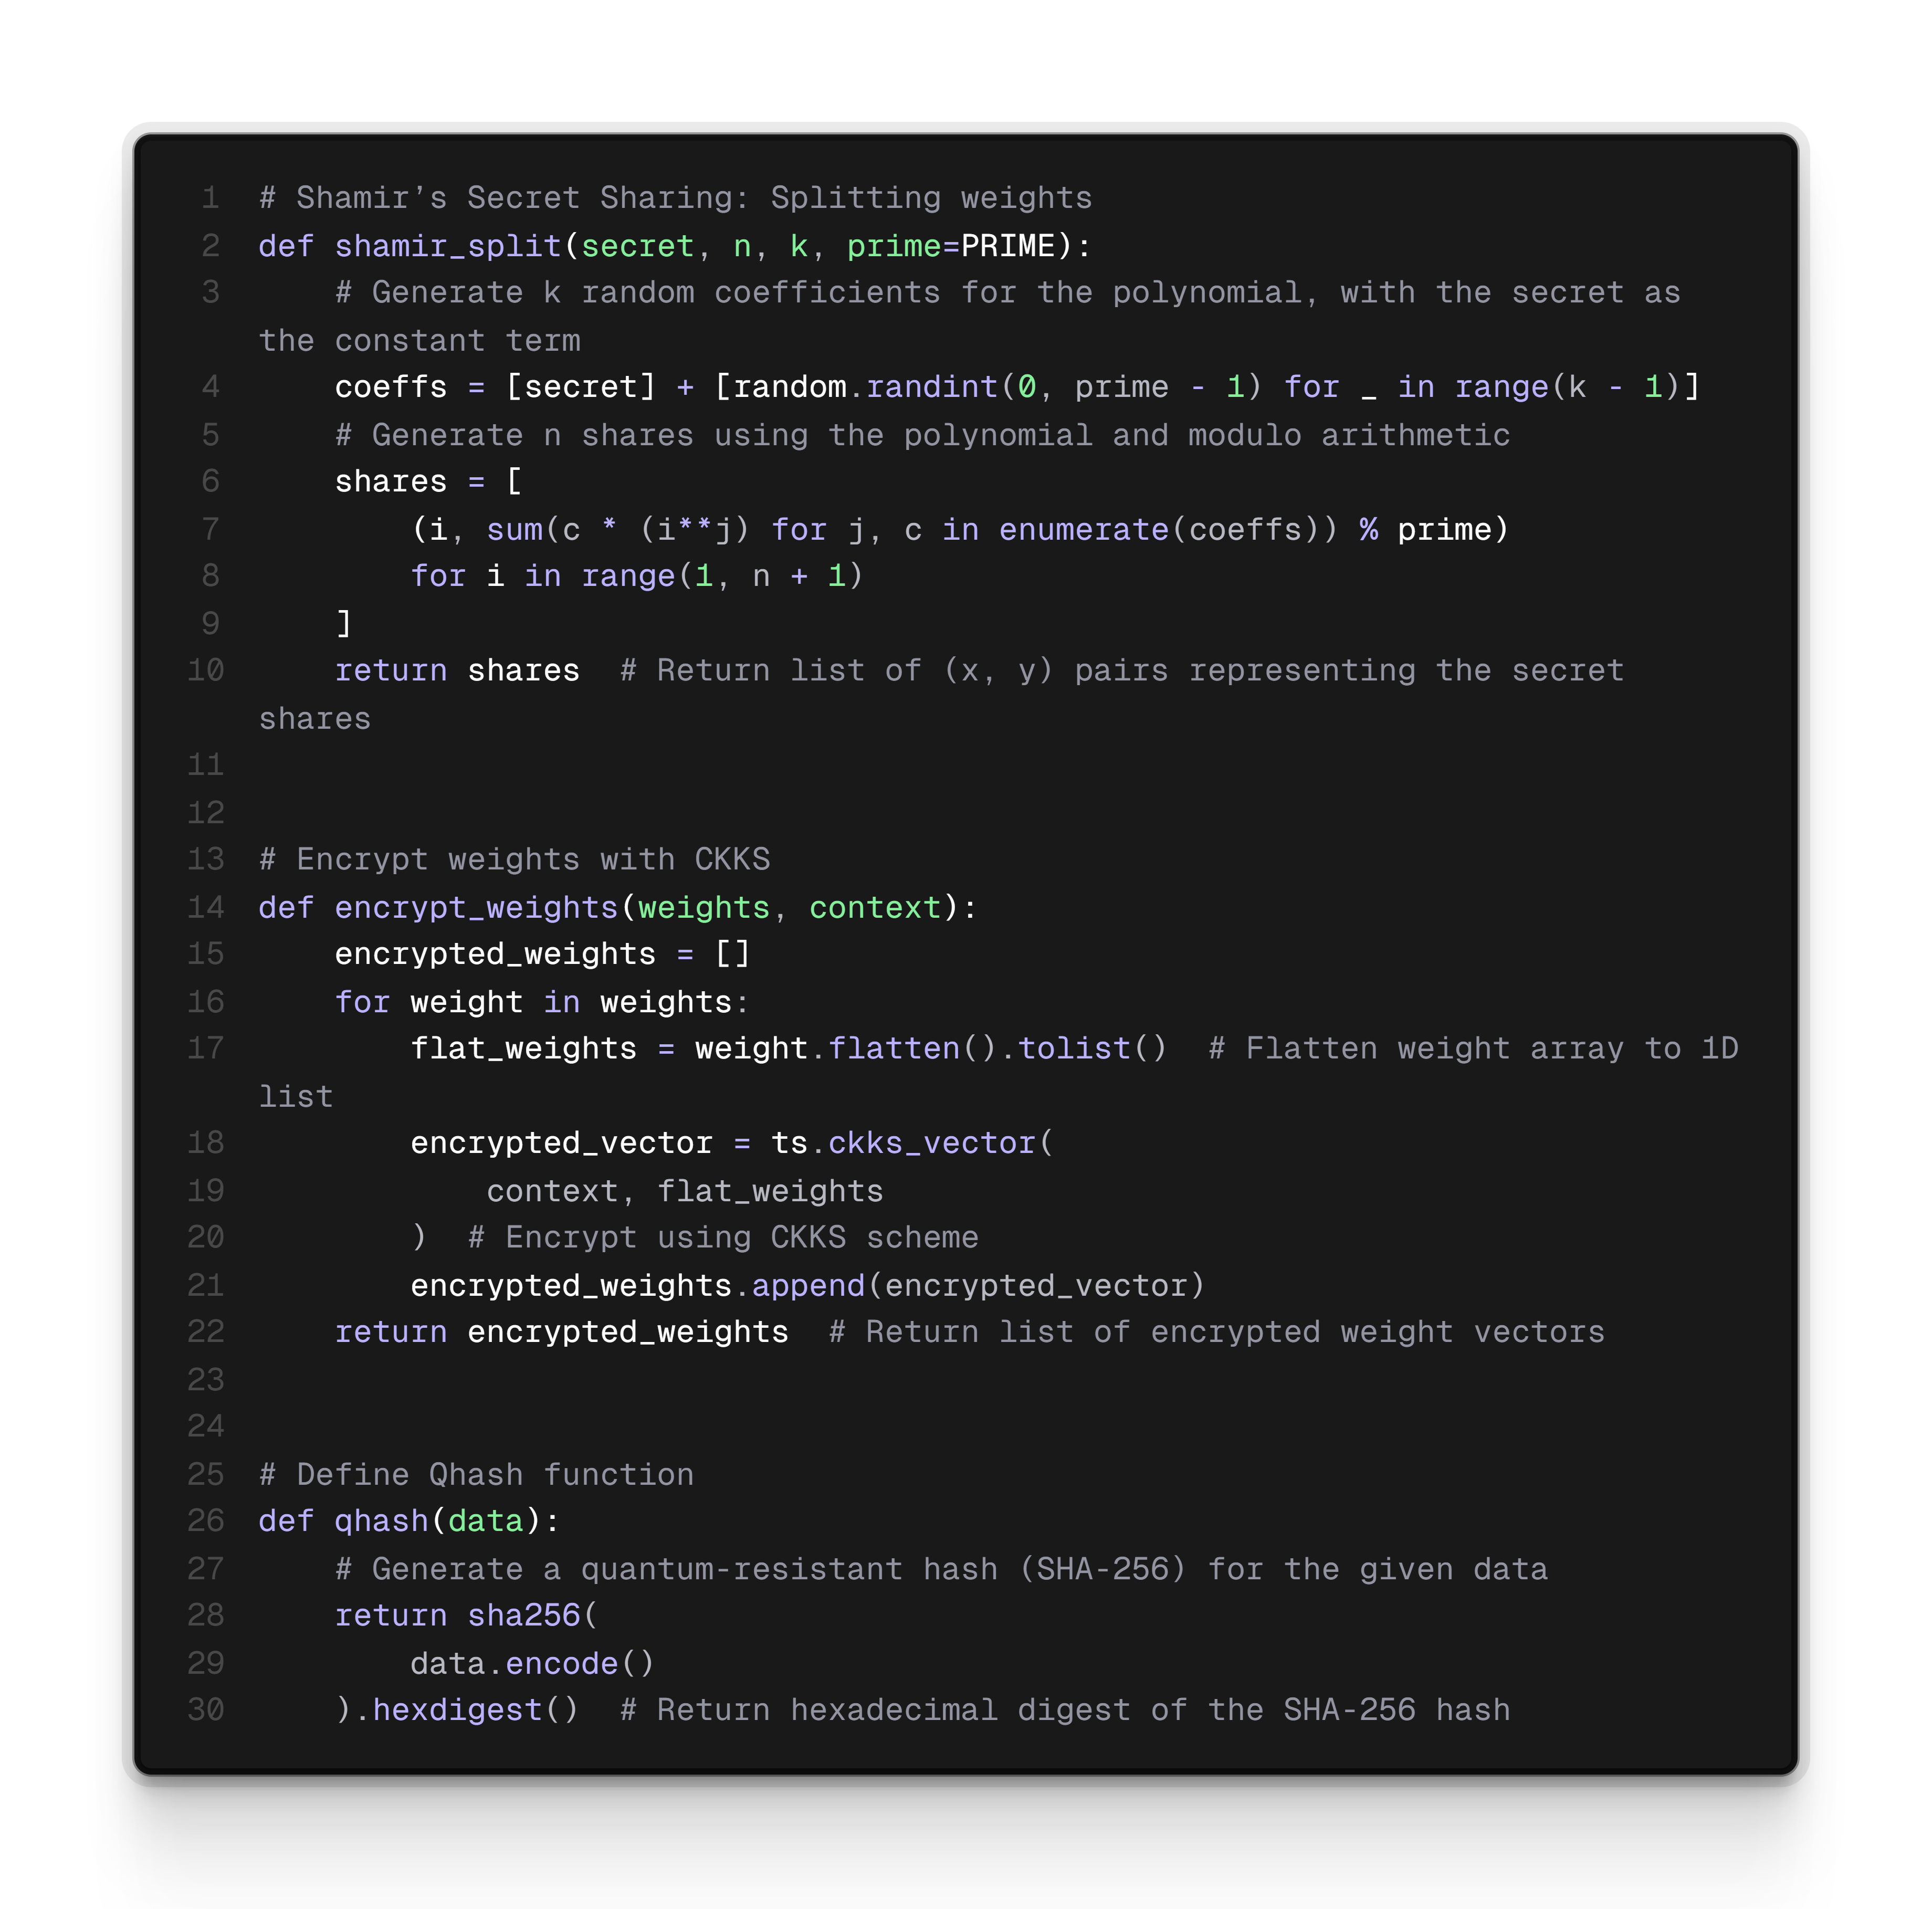
\includegraphics[height = 0.47\textheight]{img/QFL_code/1.png}
\end{figure}
\noindent The code segment implements three critical components for securing the parameters and communication of a federated learning system: Shamir’s Secret Sharing, CKKS homomorphic encryption, and a quantum-resistant hash function.\\
The function \texttt{shamir\_split(secret, n, k, prime)} is used to split model weight into $n$ distinct shares using \textbf{Shamir’s Secret Sharing} scheme. It first generates a random polynomial of degree $k-1$ with the secret as the constant term, and evaluates it at $n$ different $x$-coordinates. Each share corresponds to a unique point $(x, y)$ on this polynomial. The shares can be safely distributed to different clients or nodes. Only when at least $k$ shares are combined can the original secret be reconstructed, ensuring threshold-based access control.\\
\begin{figure}[h!]
	\centering
	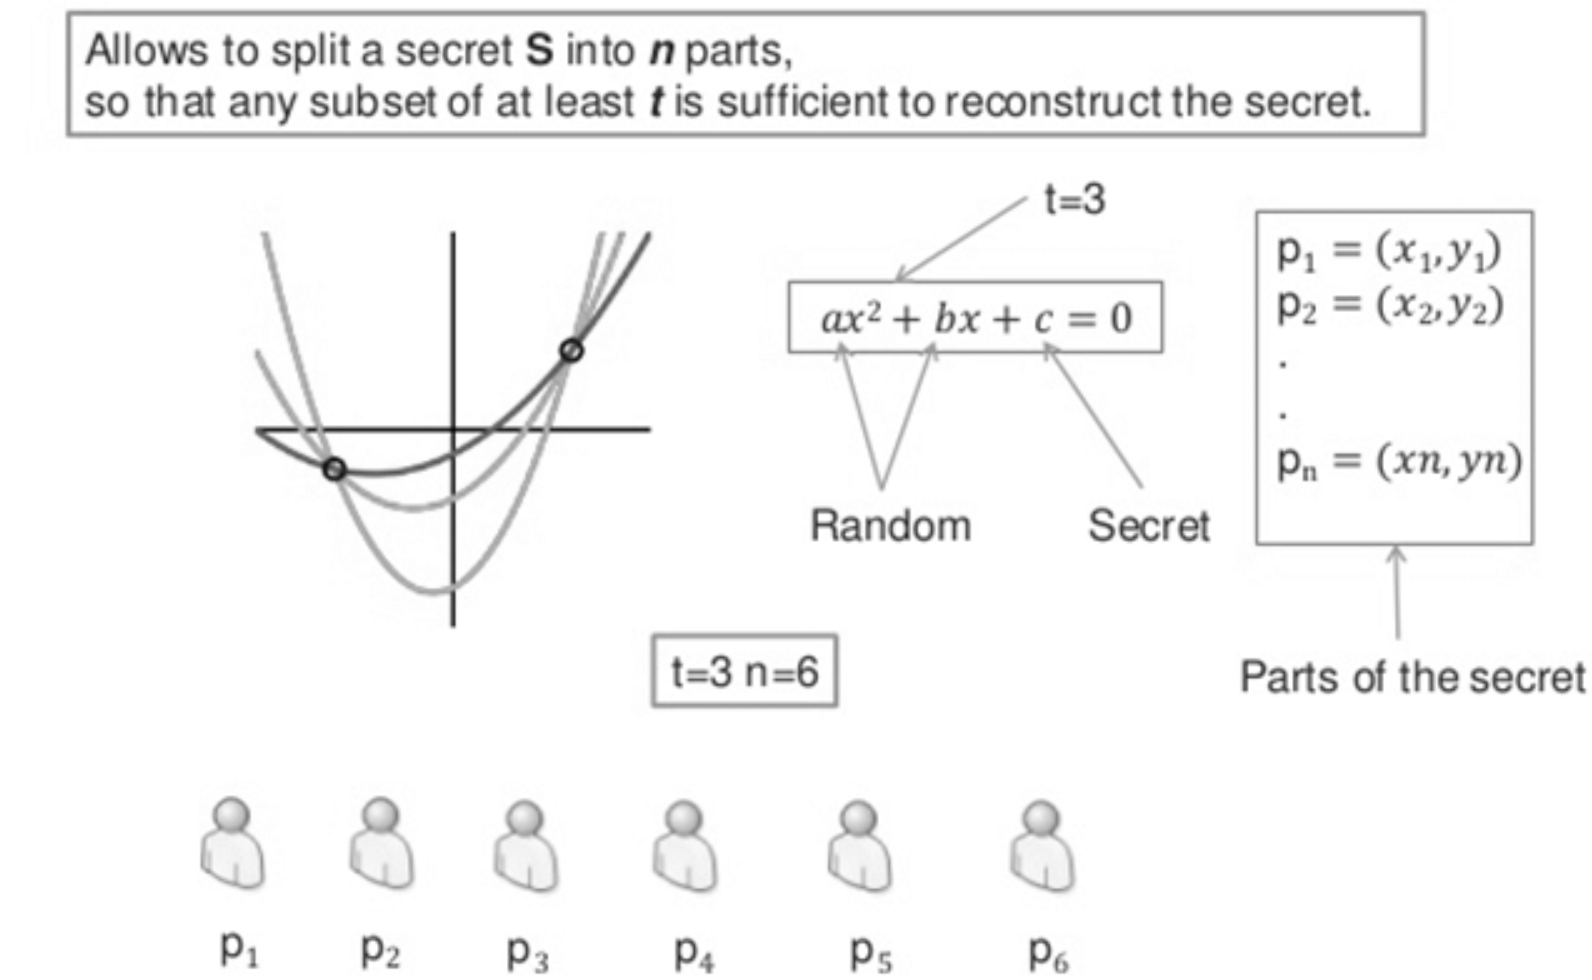
\includegraphics[height = 0.30\textheight]{img/QFL_code/SSS.png}
	\caption{Shamir's Secret Sharing Example}
\end{figure}

\noindent The \texttt{encrypt\_weights(weights, context)} function is responsible for encrypting the weights of a machine learning model using the \textbf{CKKS} (Cheon-Kim-Kim-Song) homomorphic encryption scheme. CKKS enables approximate arithmetic over encrypted real or complex numbers by encoding floating-point vectors into the coefficients of a polynomial over a cyclotomic ring. Specifically, CKKS works over a ring of the form \( \mathbb{Z}_q[X]/(X^N + 1) \), where \( N \) is a power of two and \( q \) is a large modulus. The plaintext values are first scaled by a factor \( \Delta \gg 1 \) to preserve precision, then embedded into the complex plane via a canonical embedding before encryption.\\
Each weight tensor is first flattened and converted into a list of floating-point numbers, then encrypted using the TenSEAL library's \texttt{ts.ckks\_vector} method. This method handles encoding, scaling, and encryption, using the encryption \texttt{context} to access the appropriate public keys and encryption parameters (such as polynomial degree, scale, and coefficient modulus chain). CKKS supports operations like addition and multiplication directly on encrypted data, making it particularly suitable for privacy-preserving inference in machine learning.\\
The \texttt{qhash(data)} function, on the other hand, generates a \textbf{cryptographic hash} of the input string using the SHA-256 algorithm, which produces a 256-bit digest represented in hexadecimal form. The input is first encoded into bytes before being passed to the hashing function. While SHA-256 is not strictly quantum-resistant—since Grover’s algorithm could reduce its effective security level from 256 to roughly 128 bits—it is still considered \emph{quantum-resilient} in practice for many applications. This means that even in the presence of a quantum adversary, brute-force attacks remain computationally infeasible with current and near-future quantum hardware.


\subsubsection*{- Secure Aggregation and Hashing in Federated Quantum Neural Networks}
\begin{figure}[H]
	\centering
	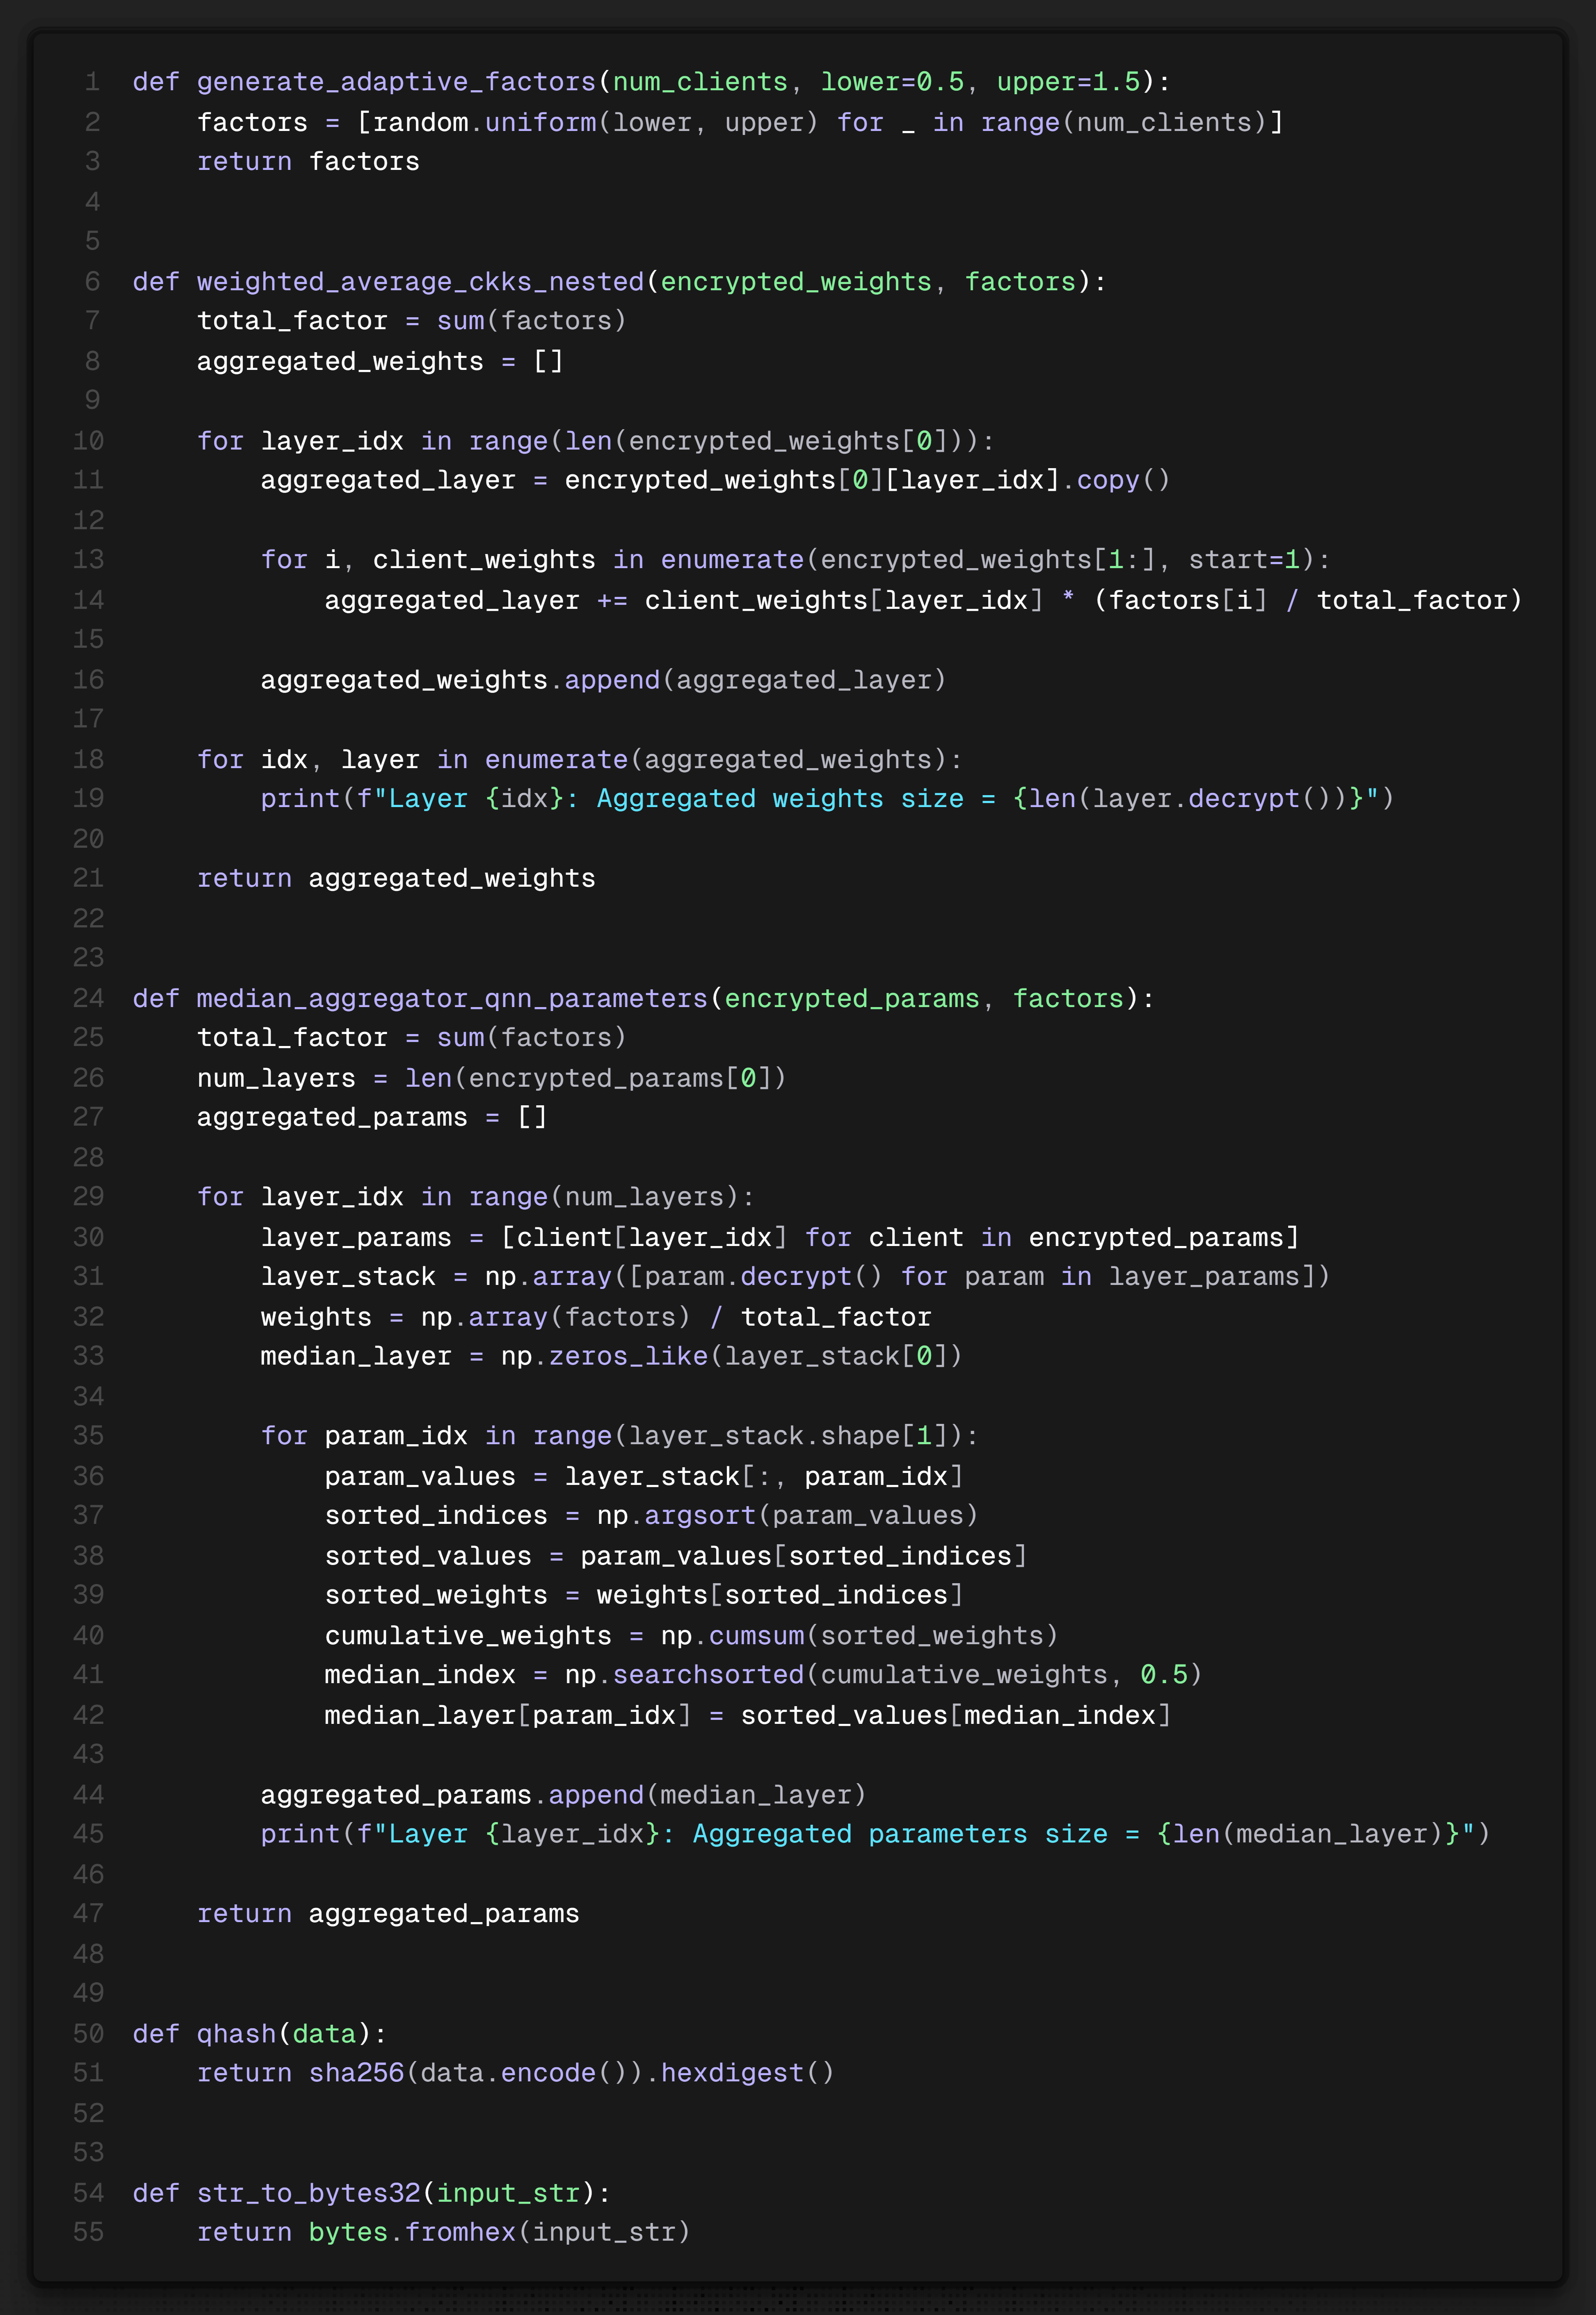
\includegraphics[height = 0.6\textheight]{img/QFL_code/2.png}
\end{figure}
\paragraph{Adaptive Weight Generation}
\texttt{generate\_adaptive\_factors(num\_clients, lower, upper)} generates a list of random floating-point values, one per client, uniformly sampled from a defined range. These values act as \textit{adaptive scaling factors} used to weight each client's contribution during aggregation. Such factors can reflect data quality, sample size, or trustworthiness of each client, and are later normalized when applied to model updates. In this case, the function results to be not so accurate, since generates random adaptive values. In a real-world scenario, these factors should be determined based on the clients' performance metrics, such as accuracy or loss on a validation set, or other criteria that reflect the quality of their local models.
\paragraph{Homomorphic Weighted Averaging}
\texttt{weighted\_average\_ckks\_nested(encrypted\_weights, factors)} performs homomorphic aggregation of encrypted model parameters. It assumes that each client's model weights are encrypted using the CKKS scheme and structured as a list of layers. For each layer, it computes a weighted sum across all clients, where each client's weights are scaled by their corresponding adaptive factor. Since the operations are performed directly on encrypted data, the aggregation process ensures strong privacy guarantees. Additionally, the code includes a diagnostic step that decrypts each aggregated layer to log its dimensionality.
\paragraph{Robust Median Aggregation}
The \texttt{median\_aggregator\_qnn\_parameters(encrypted\_params, factors)} function implements a robust aggregation mechanism for federated or distributed learning by computing the \textbf{weighted median} of model parameters instead of the standard weighted mean. This approach increases resistance to outliers or malicious clients by ensuring that the final aggregated parameter values reflect the majority trend rather than being influenced by extreme values.\\
The input \texttt{encrypted\_params} is a list of lists, where each inner list contains the encrypted parameters of a model layer from an individual client. The \texttt{factors} list contains adaptive weighting factors (e.g., based on data quality or trustworthiness) associated with each client.\\
The function proceeds as follows:
\begin{enumerate}
  \item Compute the total sum of all weighting factors, and normalize them to obtain a probability distribution over clients.
  \item Iterate over each layer index. For each layer:
  \begin{enumerate}
    \item Collect the encrypted parameters from all clients for that specific layer.
    \item Decrypt all parameters to obtain plaintext vectors.
    \item For each parameter index (i.e., position within the parameter vector):
    \begin{enumerate}
      \item Extract all client values at that position.
      \item Sort the values in ascending order, along with their associated normalized weights.
      \item Compute the cumulative sum of the sorted weights.
      \item Identify the smallest index \( i \) such that the cumulative weight exceeds 0.5. This corresponds to the \textbf{weighted median} of the parameter.
      \item Assign the median value to the corresponding position in the aggregated parameter vector.
    \end{enumerate}
  \end{enumerate}
  \item Append the aggregated (median) parameter vector for each layer to the result.
\end{enumerate}

\paragraph{Quantum-Resistant Hashing}
\texttt{qhash(data)} computes a cryptographically secure hash of an input string using the SHA-256 algorithm.


\subsubsection*{- Model Serialization, AES Encryption, and Simulated QKD}
\begin{figure}[H]
	\centering
	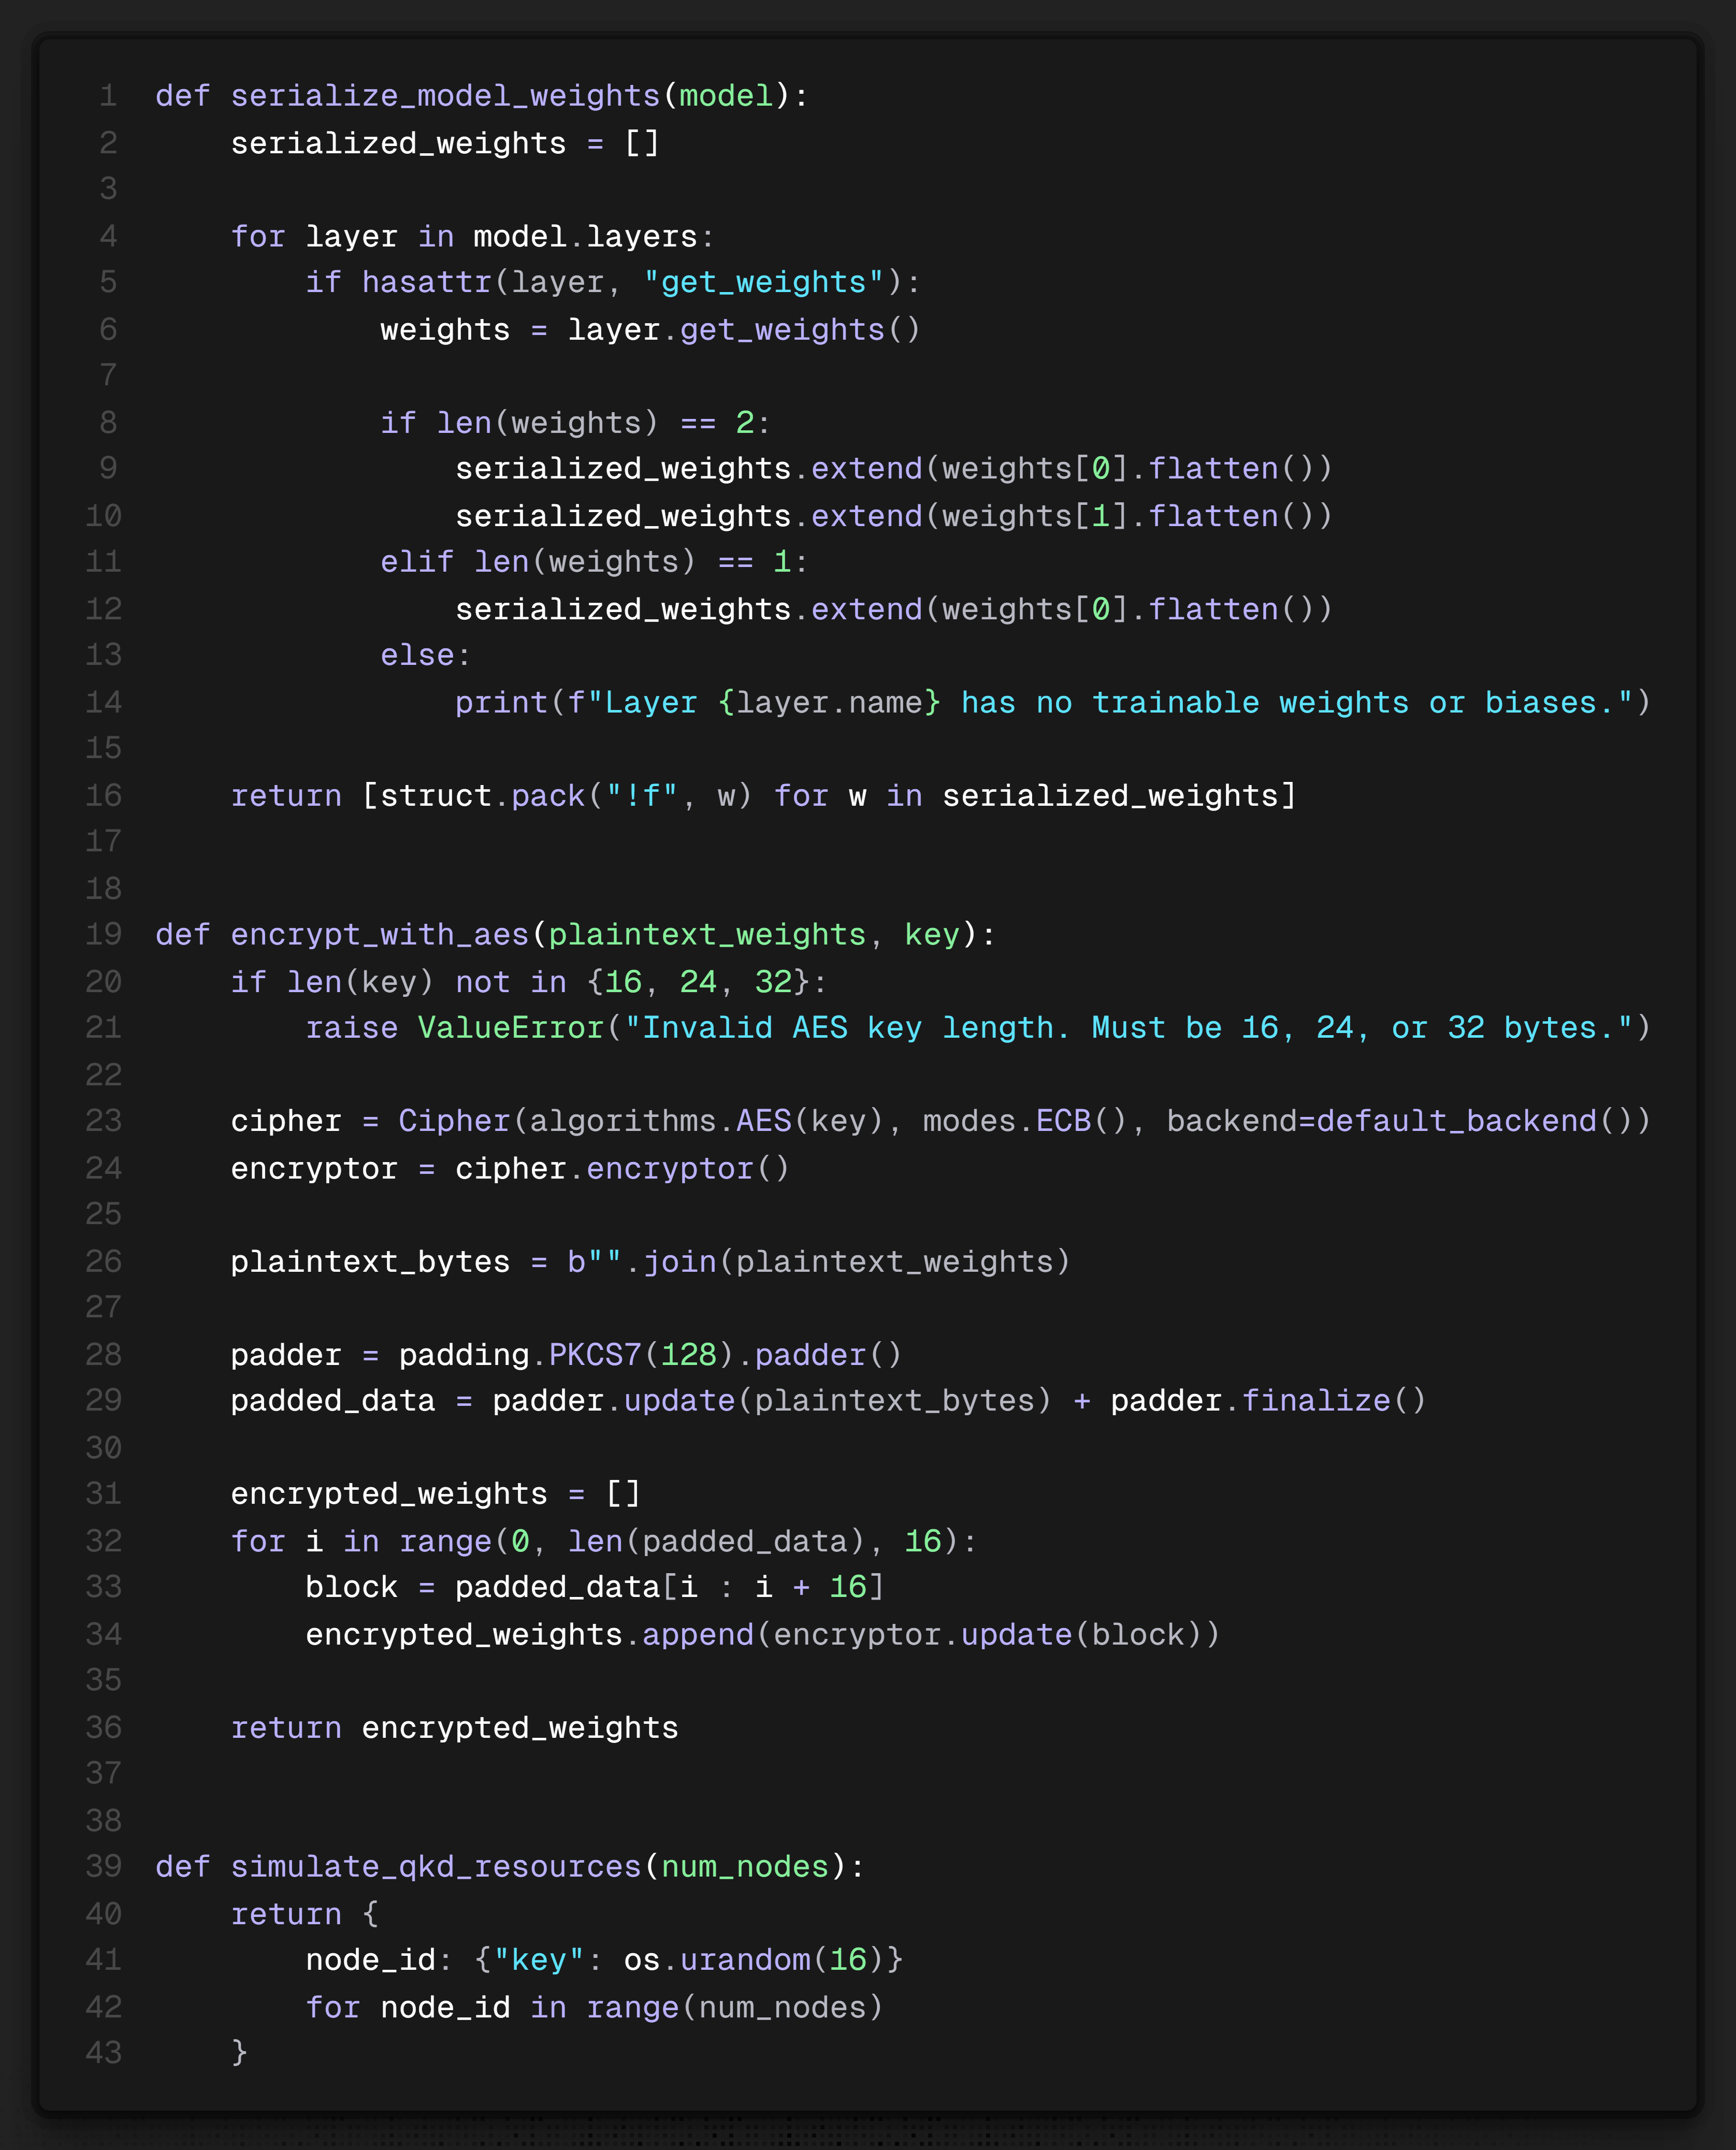
\includegraphics[height = 0.52\textheight]{img/QFL_code/3.png}
\end{figure}
This section introduces a secure pipeline for serializing and encrypting the parameters of a neural network model, along with a simulated key distribution mechanism inspired by Quantum Key Distribution (QKD).
\paragraph{AES-Based Encryption}
The \texttt{encrypt\_with\_aes(plaintext\_weights, key)} function encrypts the serialized model weights using the AES (Advanced Encryption Standard) block cipher in \textbf{Electronic Code Book (ECB)} mode. Before encryption, the input data is padded using the \textbf{PKCS\#7} padding scheme to ensure that its length is a multiple of AES’s block size (16 bytes).
\paragraph{PKCS\#7 Padding.} Let \( B = 16 \) be the AES block size in bytes, and let the length of the plaintext (in bytes) be \( L \). If \( L \mod B = r \), the plaintext is padded by appending \( B - r \) bytes, each of which has value \( B - r \). Formally, if \( P \in \{0,1\}^{L} \) is the plaintext, then the padded message is:
\[
P' = P \, \| \, \underbrace{(B - r)\|(B - r)\|\dots\|(B - r)}_{B - r \text{ times}} \in \{0,1\}^{L + (B - r)}.
\]
If the length is already a multiple of \( B \), an entire block of padding of value \( B \) is added.
\paragraph{ECB Mode.} In Electronic Code Book mode, the padded plaintext is divided into \( n \) blocks \( P'_1, P'_2, \ldots, P'_n \), each of length \( B \), and each block is encrypted independently using the AES cipher \( E_k \) with key \( k \):
\[
C_i = E_k(P'_i) \quad \text{for } i = 1, \dots, n.
\]
The resulting ciphertext is the concatenation of the encrypted blocks:
\[
C = C_1 \| C_2 \| \dots \| C_n.
\]
While ECB mode is deterministic and allows parallel encryption of blocks, it is generally \emph{not semantically secure} because identical plaintext blocks yield identical ciphertext blocks. It is suitable only when input data does not exhibit structural redundancy (e.g., fixed-format weights), or when semantic security is not a strict requirement.
\paragraph{Simulated QKD for Key Assignment}
\texttt{simulate\_qkd\_resources(num\_nodes)} simulates a Quantum Key Distribution (QKD) system by generating a unique AES key for each client or node in a distributed learning network. The function approximates the output of a QKD protocol by using \texttt{os.urandom} to generate secure, random 128-bit keys. The function returns a dictionary mapping each node identifier to its respective symmetric key.


\subsubsection*{- AES Decryption and Model Weight Deserialization}
\begin{figure}[H]
	\centering
	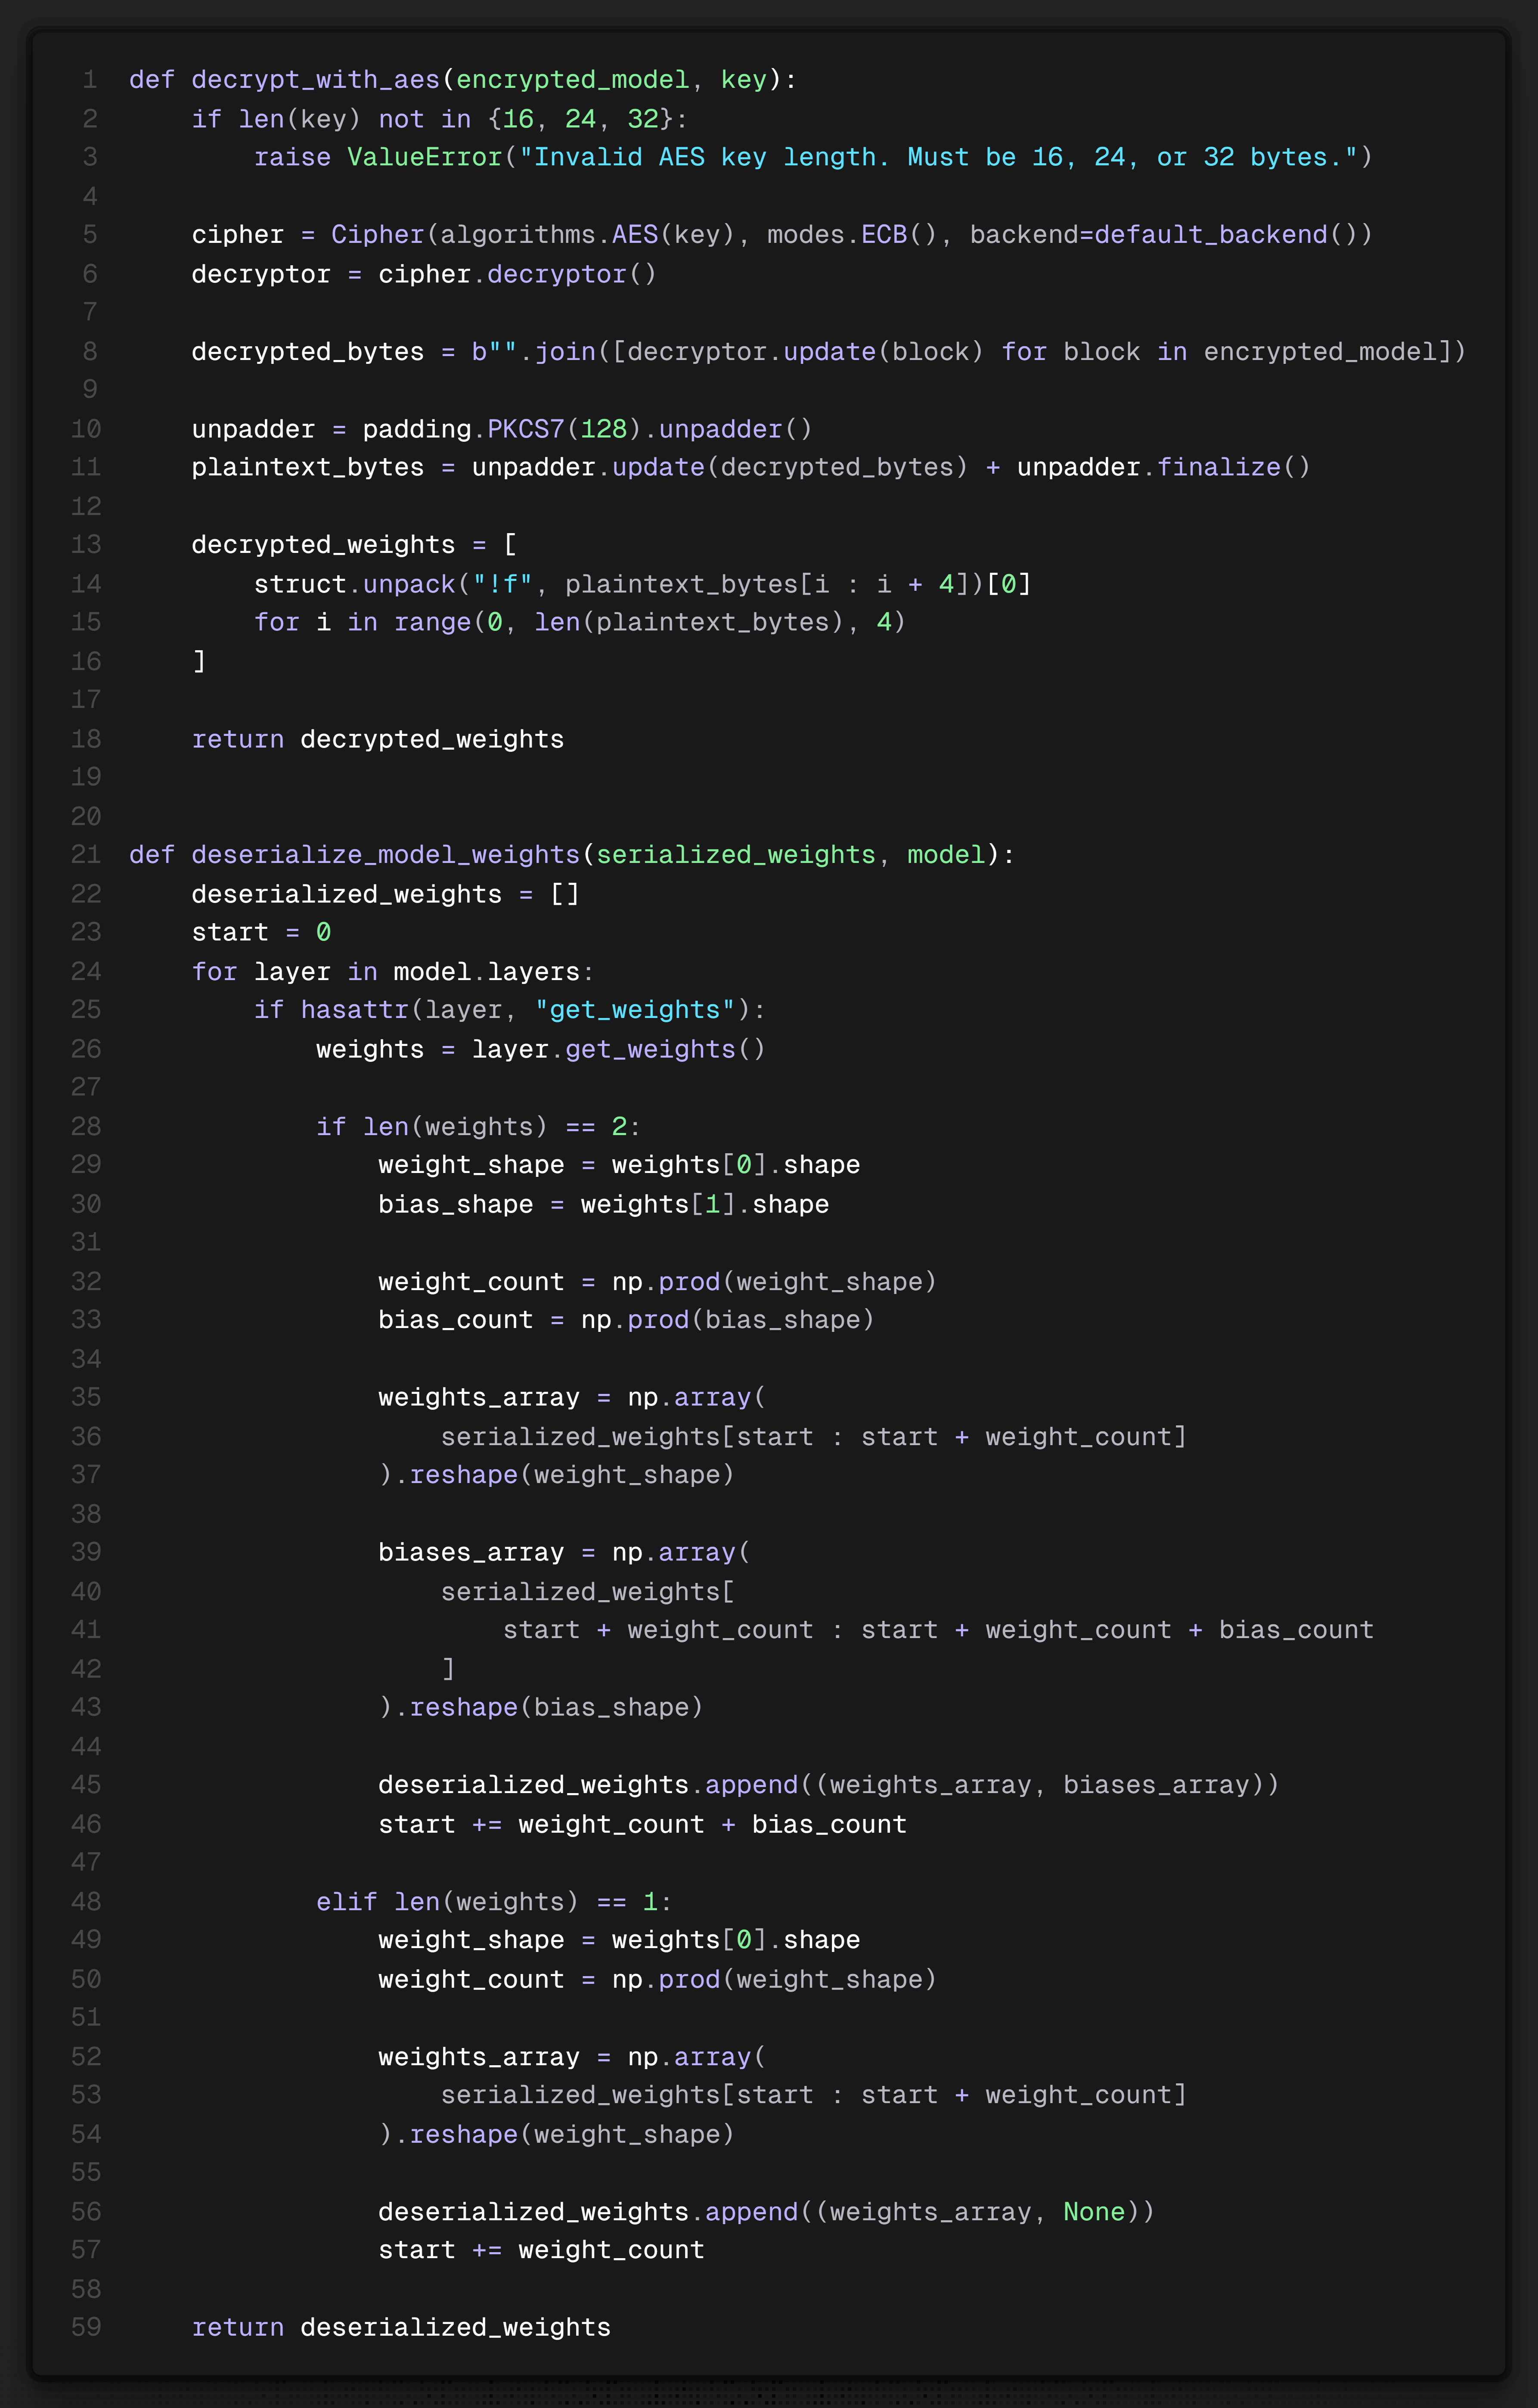
\includegraphics[height = 0.5\textheight]{img/QFL_code/4.png}
\end{figure}
To complete the secure model transmission and reconstruction pipeline, the following functions are used to reverse the encryption and flattening processes previously applied to a neural network's parameters. Specifically, they decrypt AES-encrypted model weights and reshape the flat float list back into tensors compatible with a Keras model's architecture.
\paragraph{AES Decryption of Model Weights}
\texttt{decrypt\_with\_aes(encrypted\_model, key)} is responsible for decrypting a list of AES-encrypted 16-byte blocks. It uses the same symmetric key originally used for encryption and operates in ECB mode. The decryption process begins by concatenating the output of each decrypted block into a single byte string. Since padding was applied during encryption using the PKCS7 scheme, it is removed here to recover the original plaintext size. The raw byte stream is then parsed into 4-byte segments and converted back into 32-bit floating-point values using the \texttt{struct.unpack("!f", ...)} method. The result is a flat list of float values representing the model's parameters.
\paragraph{Weight Deserialization and Model Reconstruction}
\texttt{deserialize\_model\_weights(serialized\_weights, model)} reconstructs the original model weight tensors from a flat list of floating-point values. It assumes that the order and count of weights and biases were preserved during serialization. For each trainable layer in the Keras model, it retrieves the expected shapes of the weights and biases using \texttt{layer.get\_weights()}. It then extracts the appropriate number of elements from the flat list and reshapes them into tensors using NumPy. These are appended as tuples: either \texttt{(weights, biases)} if both exist, or \texttt{(weights, None)} if the layer has no bias terms. A running pointer ensures that the deserialization proceeds sequentially without loss or duplication of data.



\subsubsection*{- Updating Client Models with Global Weights}
\begin{figure}[H]
	\centering
	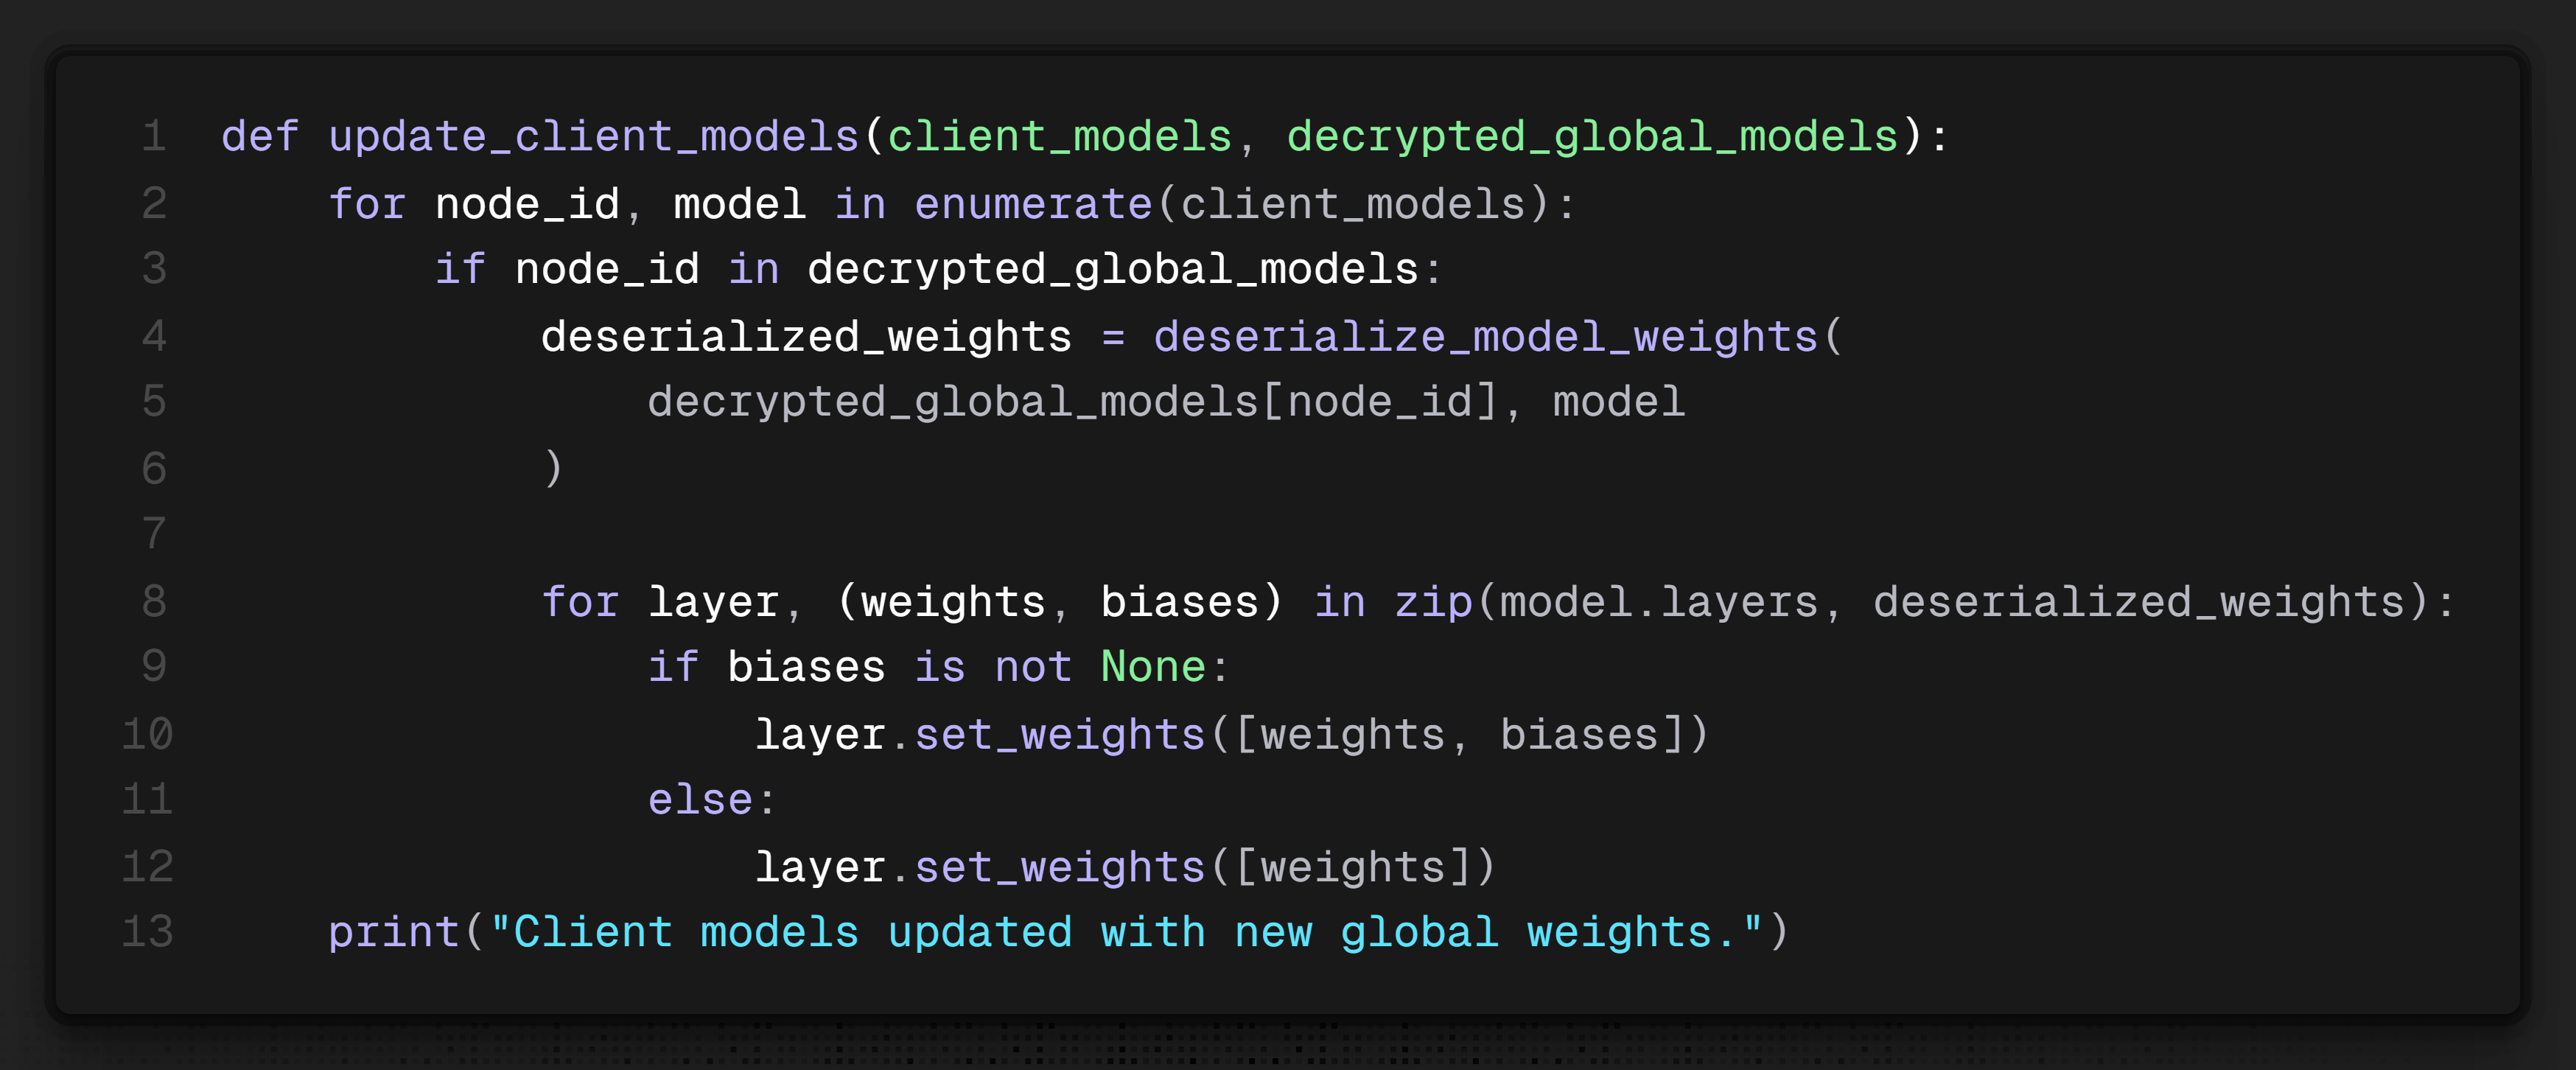
\includegraphics[height = 0.2\textheight]{img/QFL_code/5.png}
\end{figure}
Once the global model weights have been securely aggregated, encrypted, transmitted, and subsequently decrypted by individual clients, the final step is to apply these weights to each client's local model.\\
\texttt{update\_client\_models(client\_models, decrypted\_global\_models)} performs this update process by assigning the appropriate version of the decrypted global model to each client.
Each entry in the \texttt{client\_models} list represents a separate Keras model instance maintained by a client node. The dictionary \texttt{decrypted\_global\_models} maps node IDs to their corresponding sets of decrypted and flattened model weights.


\subsubsection*{- Quantum Layer Structure}
The structure used here is the same as that employed in the QNN. In particular, we use the custom 'long' layer previously described. To avoid redundancy, we refer the reader to the preceding section for a detailed explanation of the quantum layer structure and its implementation.


\subsubsection*{- Local Quantum Model}
\begin{figure}[H]
	\centering
	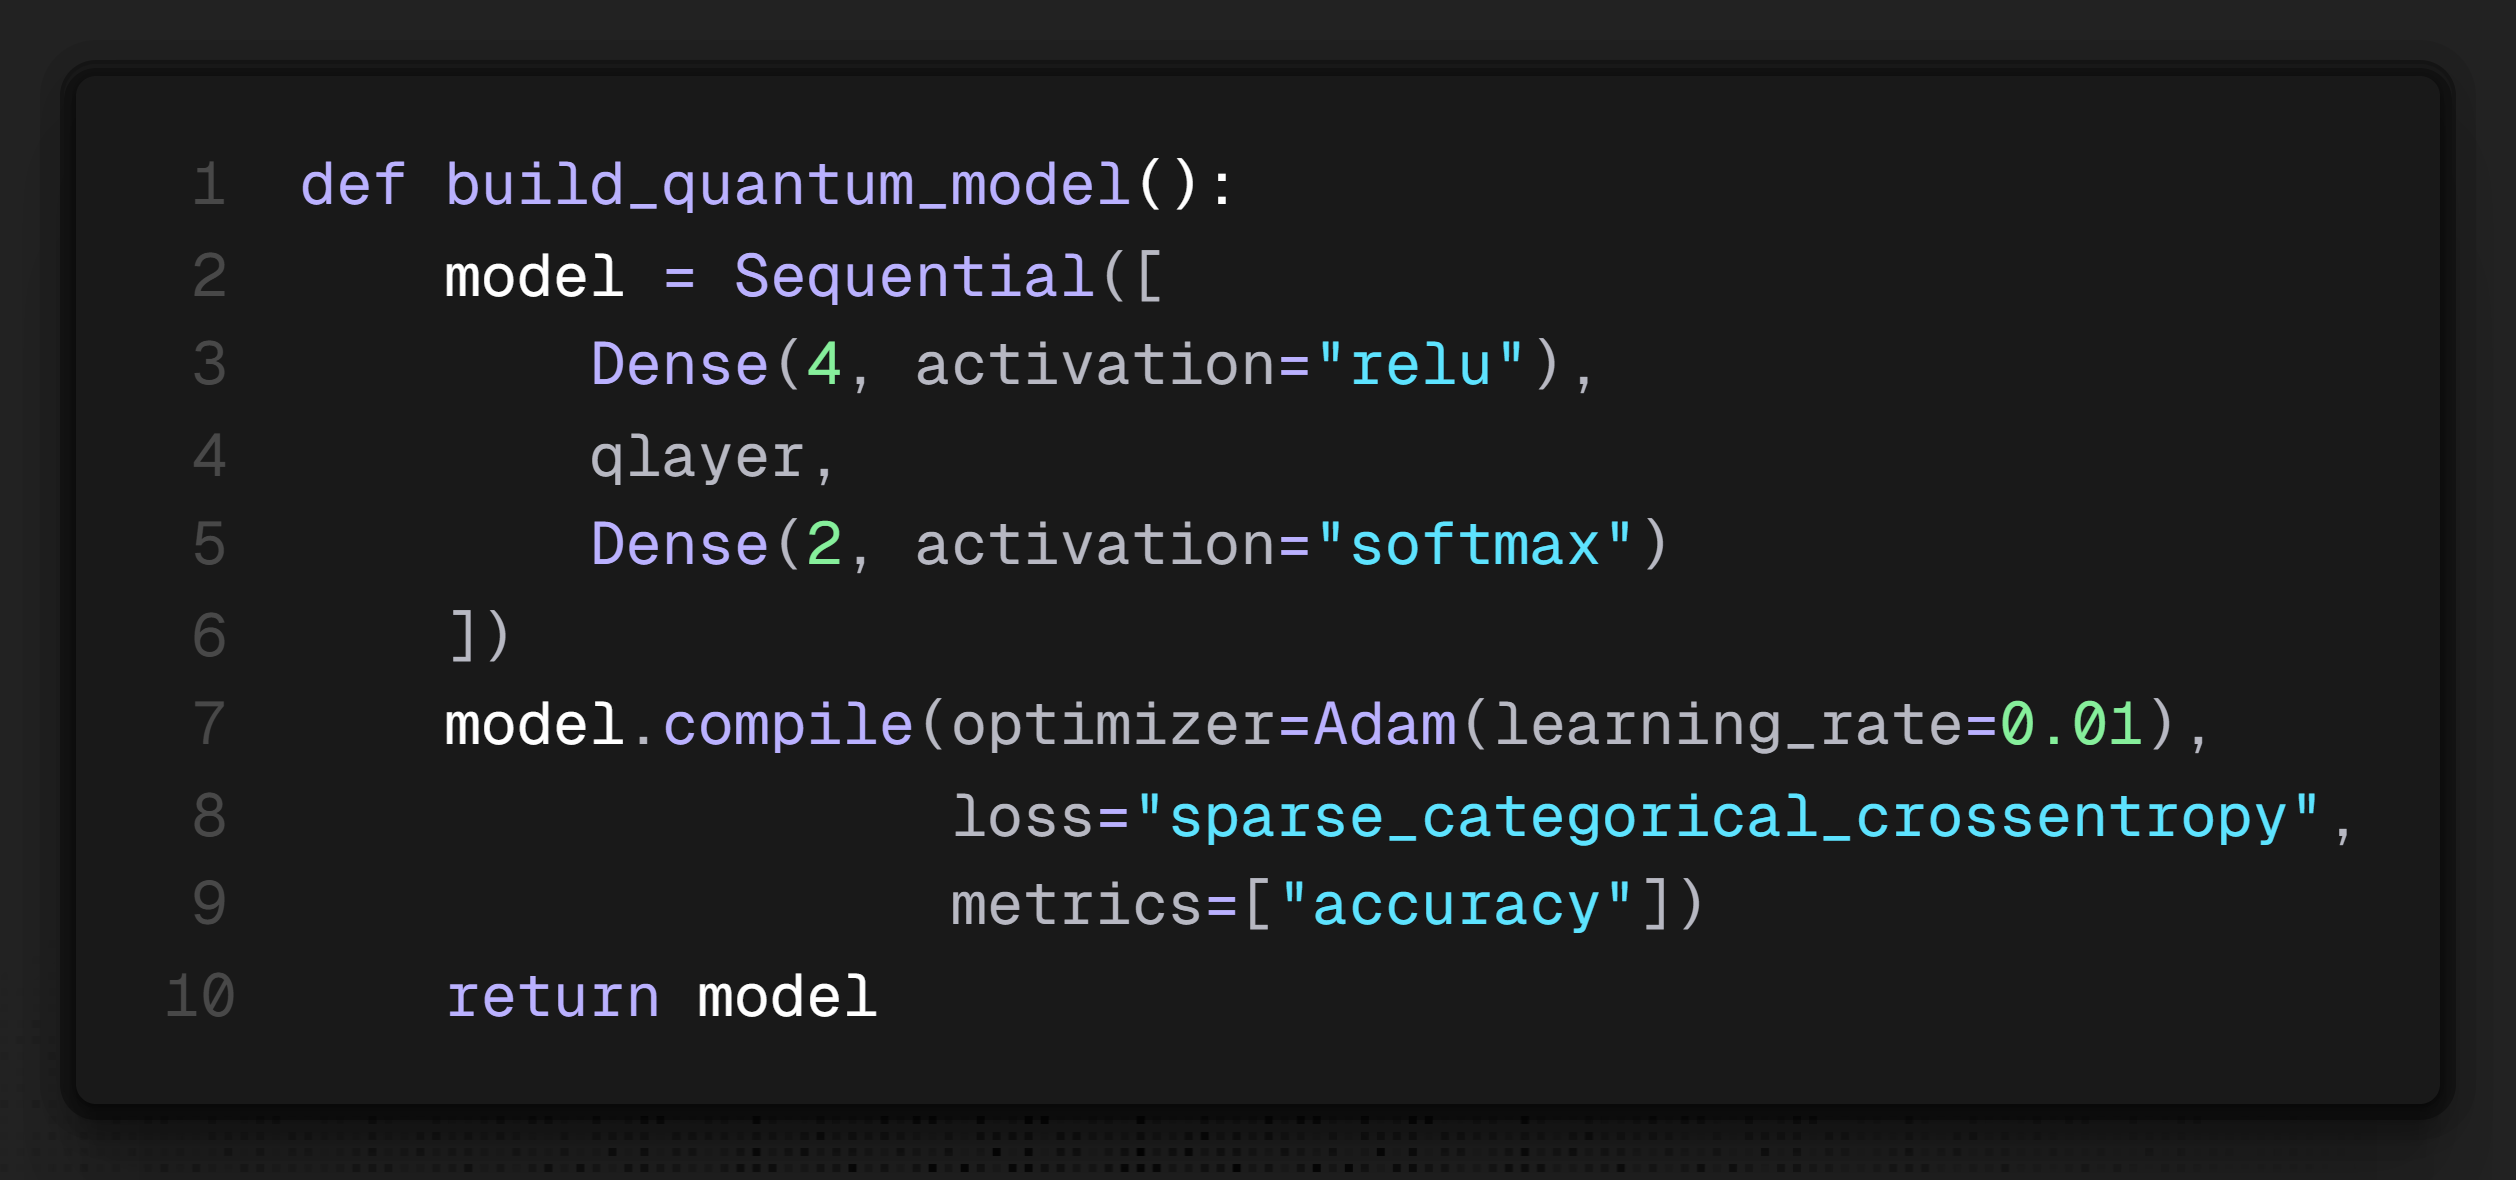
\includegraphics[height = 0.2\textheight]{img/QFL_code/6.png}
\end{figure}
The function \texttt{build\_quantum\_model()} constructs a hybrid neural network model that integrates classical dense layers with a trainable quantum layer.
The model architecture consists of three main components:
\begin{itemize}
	\item \texttt{Dense(4, activation="relu")} is the first classical layer with 4 neurons and ReLU activation. This layer performs a nonlinear transformation on the input data and projects it into a higher-dimensional space suitable for quantum processing.
	\item \texttt{qlayer} is a quantum layer instantiated using \texttt{qml.qnn.KerasLayer}, which wraps a quantum circuit defined via a QNode. This layer accepts classical input, encodes it into quantum states (e.g., via AngleEmbedding), applies the trainable quantum circuit (such as \texttt{custom\_layer\_long}), and returns classical output via expectation measurements.
	\item \texttt{Dense(2, activation="softmax")} is the final classical layer that maps the quantum output to a 2-dimensional vector suitable for binary classification. The \texttt{softmax} activation ensures that the outputs are normalized and interpretable as class probabilities.
\end{itemize}
The model is compiled using the Adam optimizer with a learning rate of 0.01, and it employs the categorical cross-entropy loss function.
In the next step, we will implement the local training process for each client.

\paragraph{Secure Weight Extraction and Encryption.}
After local training, the weights of each client's model are extracted specifically from the dense layers. These weights are first split using Shamir’s Secret Sharing scheme, which converts each real-valued weight into a set of $n$ modular shares using a polynomial of degree $k - 1$. This ensures that the weight can only be reconstructed if at least $k$ out of $n$ shares are collected. The integer conversion via multiplication by $10^6$ maintains precision while ensuring compatibility with modular arithmetic over a prime field.
Subsequently, the original weight matrices are also encrypted using the CKKS (Cheon–Kim–Kim–Song) homomorphic encryption scheme. This encryption allows computation directly on ciphertexts, meaning that model aggregation and analysis can be performed securely without decryption.
\begin{figure}[H]
	\centering
	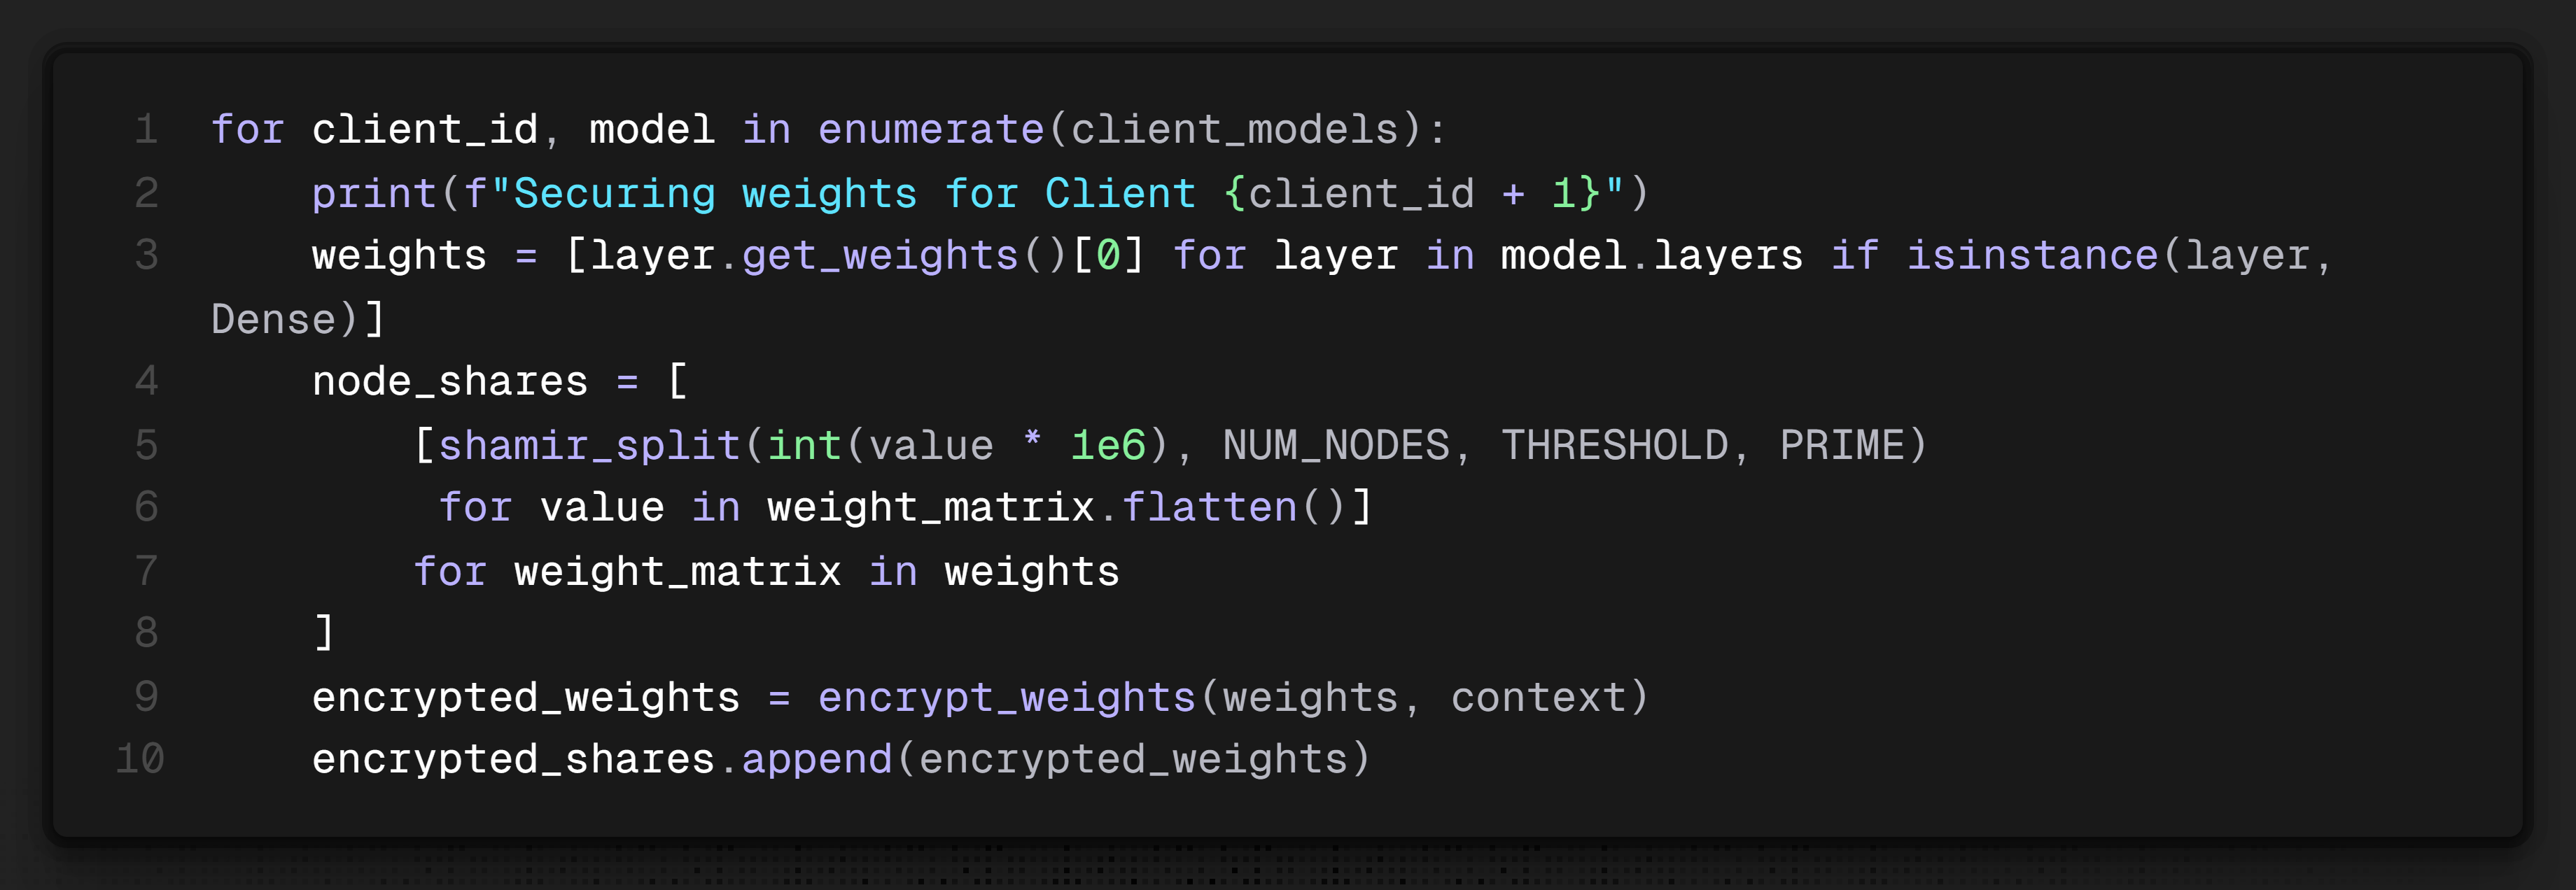
\includegraphics[height = 0.2\textheight]{img/QFL_code/7.png}
\end{figure}


\paragraph{Homomorphic Aggregation via Weighted Median.}
To construct a new global model from the encrypted local updates, a weighted median aggregation is performed directly in the encrypted domain. Each client's contribution is scaled using an adaptive factor, which reflects dynamic properties such as data quality, trust level, or sample size.\\
The encrypted weights are first decrypted temporarily (within the secure enclave of the aggregation server) to perform the median operation. For each position in the weight vector, values from all clients are collected, sorted, and the weighted cumulative distribution is computed. The value corresponding to the median weight threshold (typically at cumulative weight $\geq 0.5$) is then selected as the aggregate for that parameter. This robust aggregation reduces the influence of outliers or malicious updates while preserving differential weight importance.
\begin{figure}[H]
	\centering
	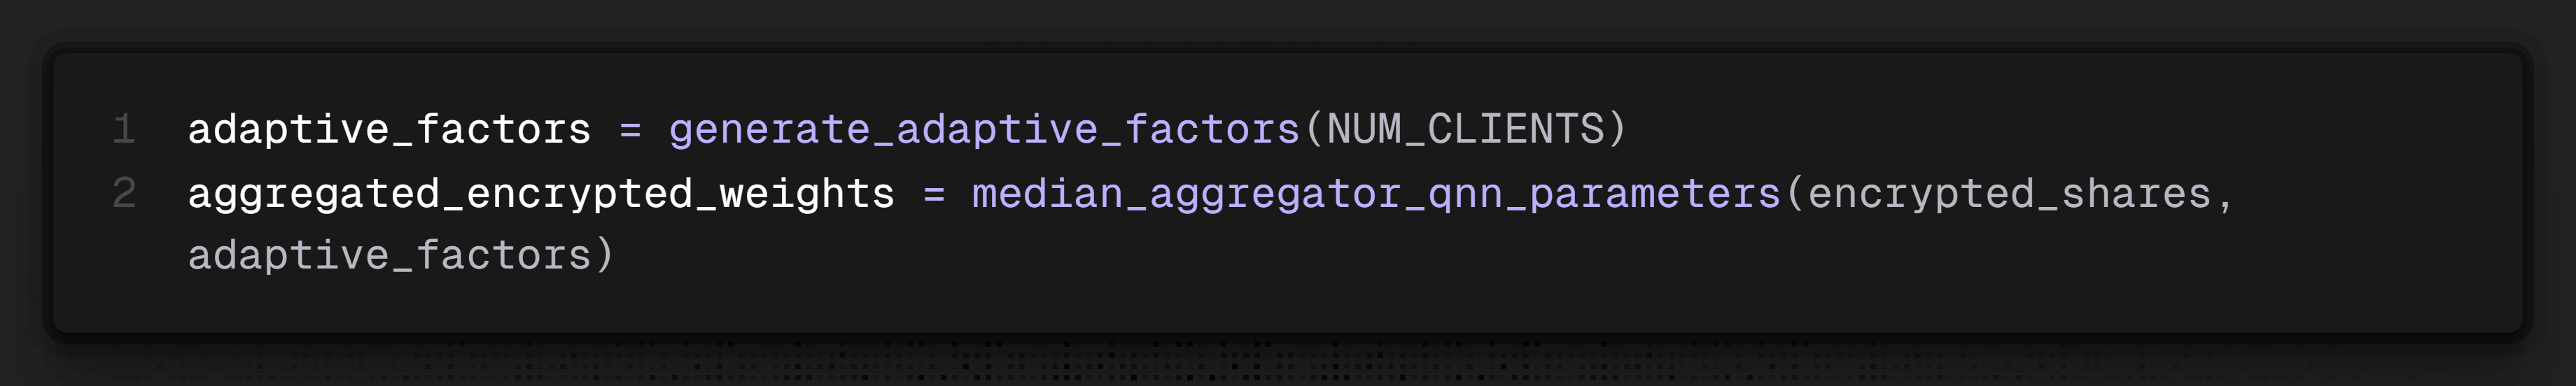
\includegraphics[height = 0.08\textheight]{img/QFL_code/9.png}
\end{figure}

\paragraph{Simulated QKD and AES-Based Model Distribution.}
To securely distribute the newly aggregated global model to all clients, a Quantum Key Distribution (QKD) simulation is employed. In this setup, each client is assigned a unique 128-bit AES key generated via a secure random process. Although not a true quantum system, this approach mimics the security properties of QKD by assuming an independent, pre-shared key per node.
The global model is serialized into 32-bit floats and encrypted block-wise using AES in ECB mode with PKCS7 padding. This encryption guarantees that only the intended client, with access to its unique key, can decrypt and load the model update.
\begin{figure}[H]
	\centering
	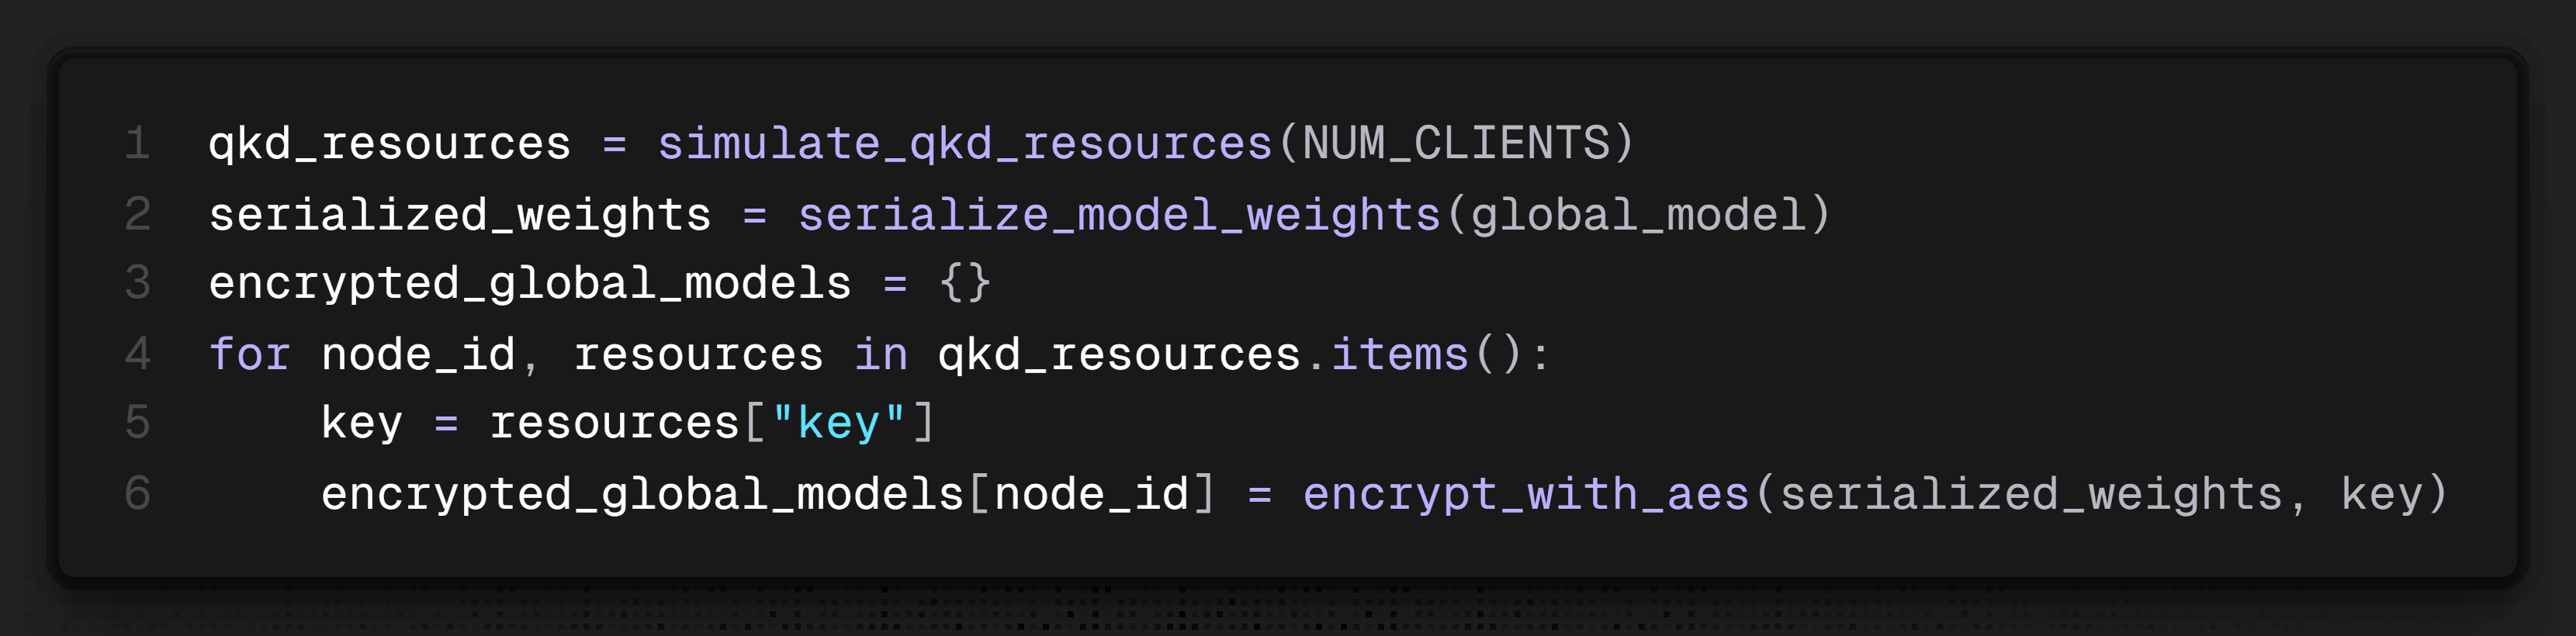
\includegraphics[height = 0.15\textheight]{img/QFL_code/10.png}
\end{figure}

\paragraph{Evaluation of Aggregated and Local Models.}
After each training and aggregation round, the global model is evaluated on a test set consisting of all clients’ data. This provides a comprehensive metric of generalization across the entire system. Simultaneously, the performance of an individual client (typically Client 1) is also assessed on its own local test set to monitor personalized model performance.
The results from each iteration are stored for both global and local accuracy, enabling longitudinal analysis of the model's evolution, convergence behavior, and fairness across clients.

\subsection{Ganache Blockchain}
Ganache is a local Ethereum blockchain emulator used primarily for testing and development of smart contracts. It allows developers to deploy and interact with contracts in a controlled environment without requiring access to the main Ethereum network. In our project, Ganache is used to simulate the blockchain environment in which the \texttt{NewSecureAggregation.sol} smart contract is deployed and tested. The Python script \texttt{deploy\_contract.py} establishes a connection to the Ganache RPC server, loads the compiled contract's ABI and bytecode, and performs the deployment using Web3.py. This setup facilitates rapid development and debugging of Ethereum-based applications.
\begin{figure}[H]
	\centering
	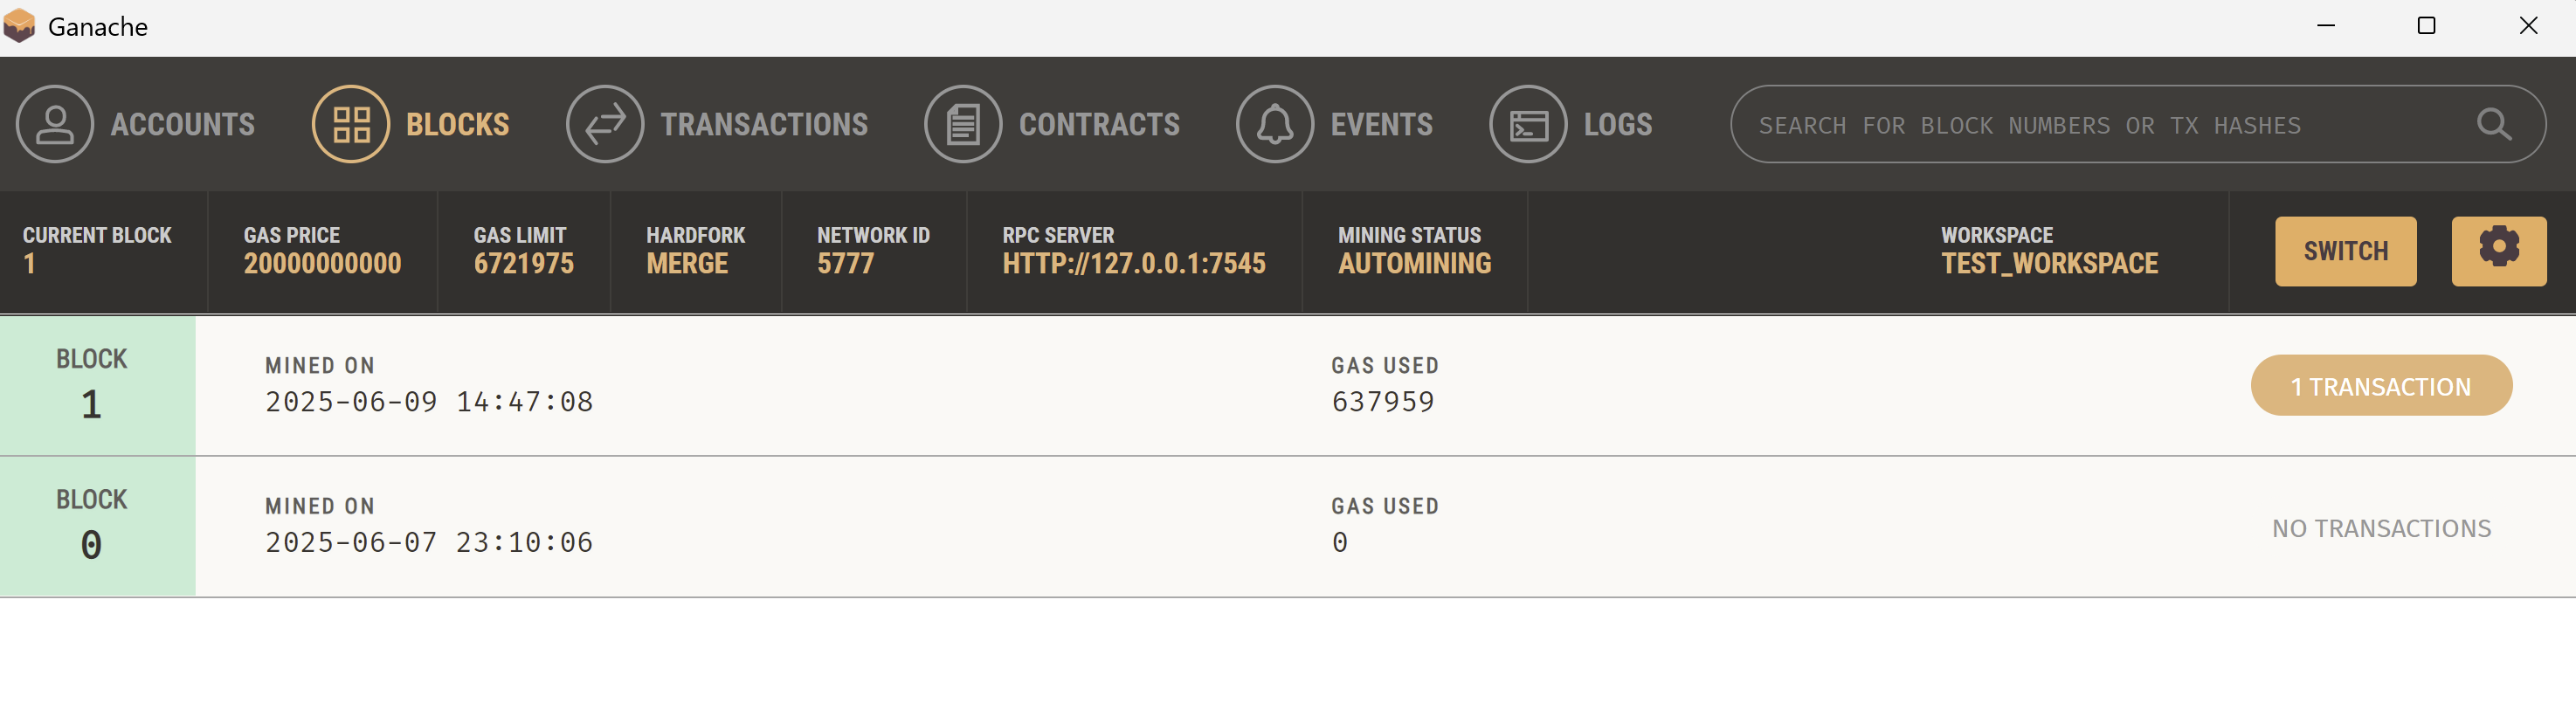
\includegraphics[height = 0.20\textheight]{img/QFL_code/Ganache.png}
\end{figure}
\subsubsection*{Smart Contract}
The \texttt{NewSecureAggregation.sol} file contains a Solidity smart contract designed to perform secure data aggregation on the Ethereum blockchain. The contract implements logic for receiving, managing, and aggregating encrypted data or model updates from multiple participants, which is particularly relevant in federated learning or privacy-preserving computation scenarios. It defines key structures such as mappings to store individual contributions and control logic to ensure that only authorized or valid data submissions are accepted. The contract may also include aggregation functions, state management, and event logging to provide transparency and auditability of operations. Its design ensures decentralization, integrity, and traceability of the aggregation process in a trustless environment.

\subsection{Results}
\begin{figure}[H]
    \centering
    \begin{minipage}{0.49\textwidth}
        \centering
        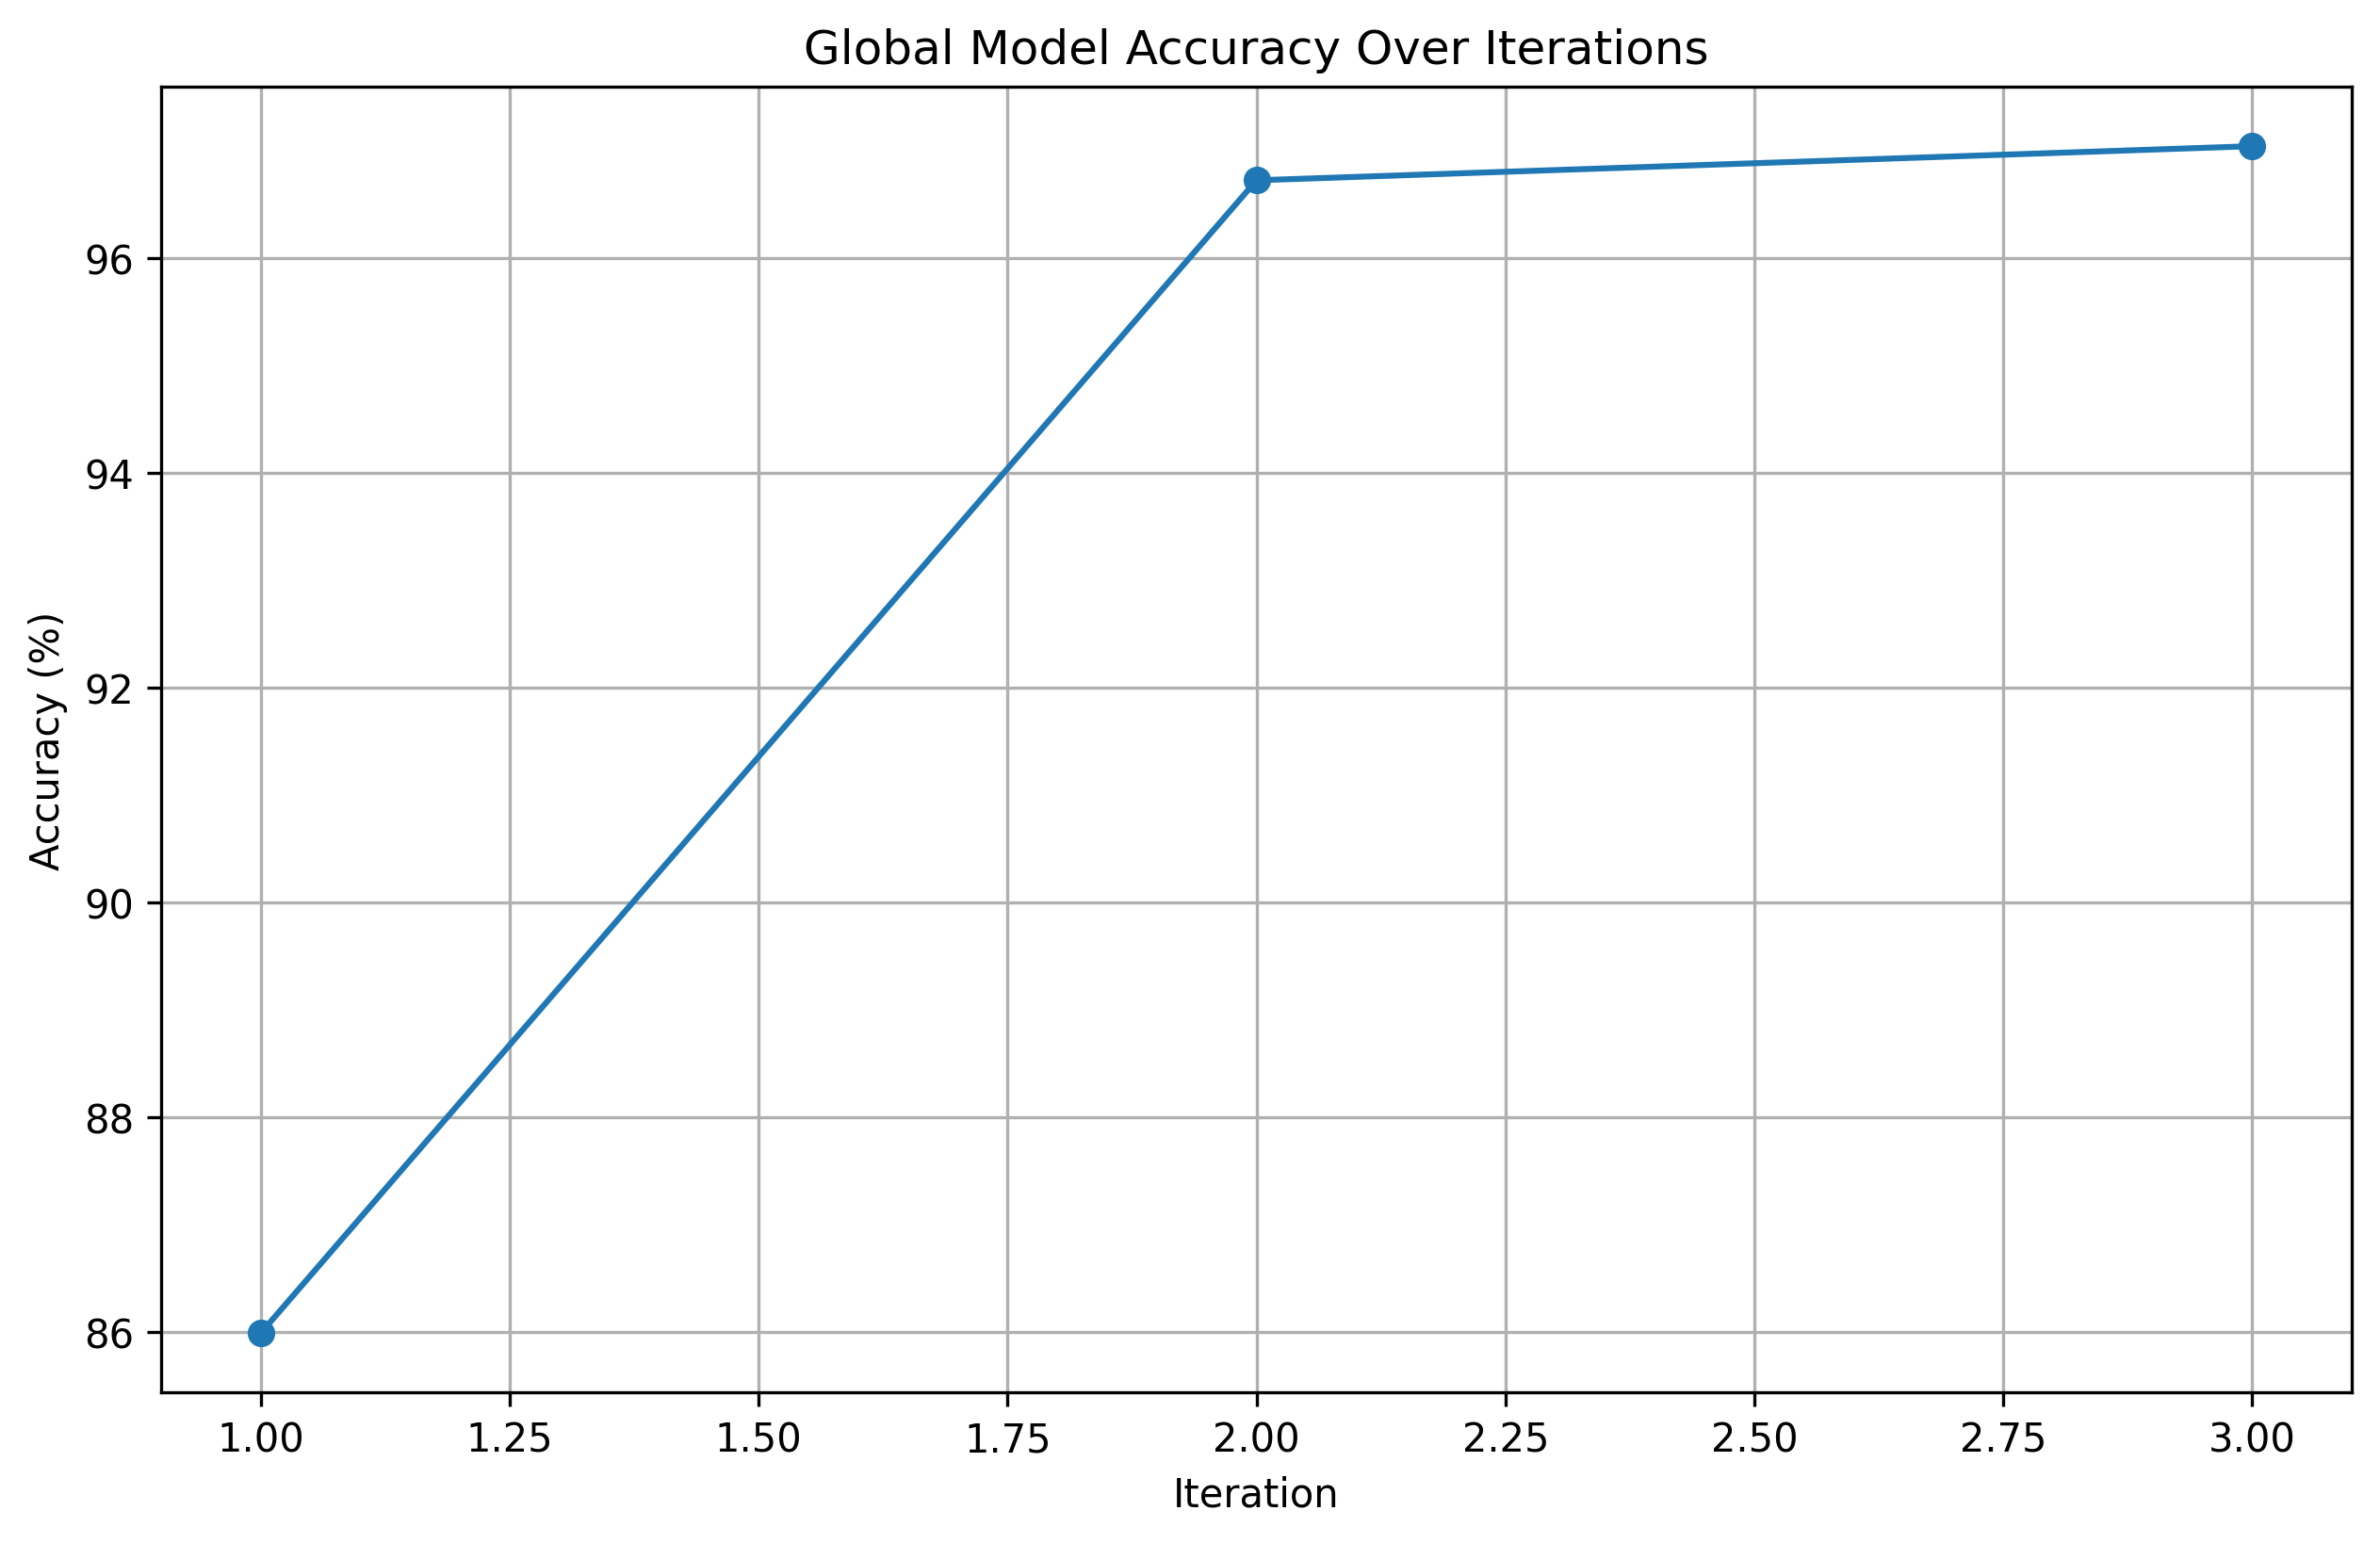
\includegraphics[height=0.23\textheight]{img/global_model_accuracy.png}
        \caption{Global model accuracy on combined test set is 97.04\%}
        \label{fig:global_accuracy}
    \end{minipage}
    \hfill
    \begin{minipage}{0.49\textwidth}
        \centering
        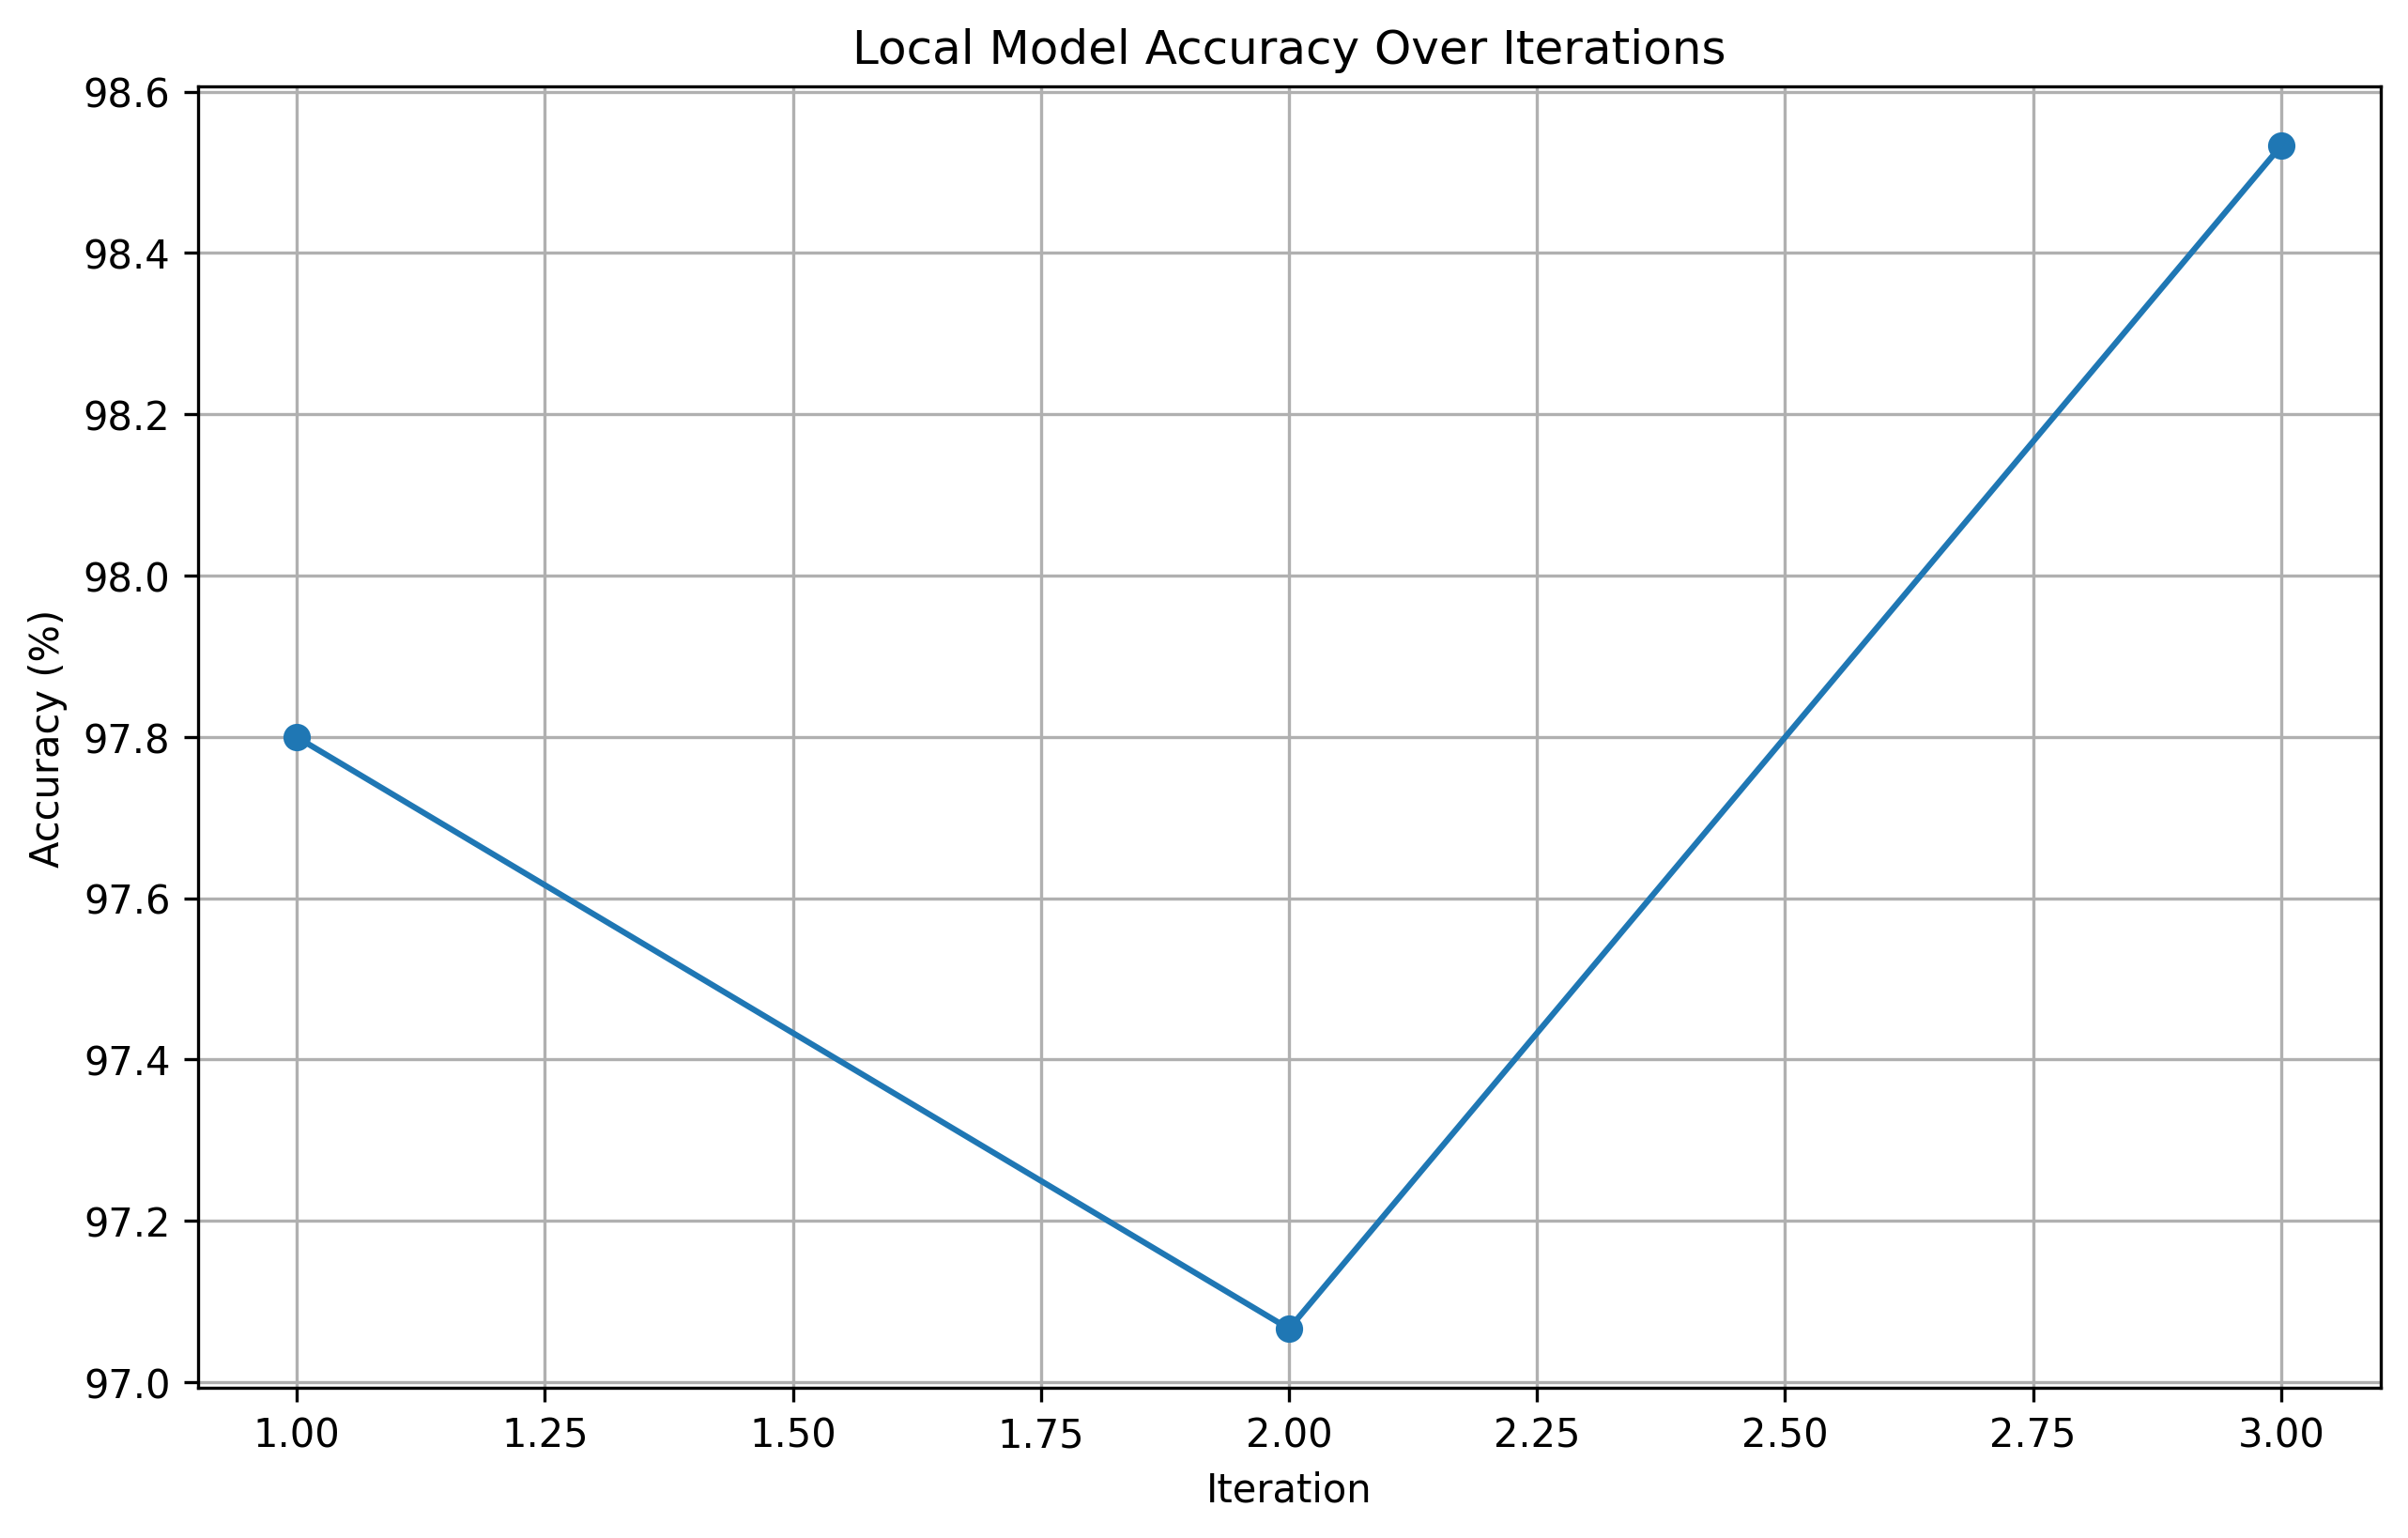
\includegraphics[height=0.23\textheight]{img/local_model_accuracy.png}
        \caption{Client 1 model accuracy on its own test set is 95.84\%}
        \label{fig:local_accuracy}
    \end{minipage}
\end{figure}

\begin{table}[H]
\centering
\begin{tabular}{|c|c|}
\hline
\textbf{Client} & \textbf{Accuracy (\%)} \\
\hline
Client 1 & 95.84 \\
Client 2 & 97.80 \\
Client 3 & 97.07 \\
Client 4 & 96.82 \\
Client 5 & 98.04 \\
Client 6 & 97.07 \\
Client 7 & 96.82 \\
Client 8 & 96.58 \\
Client 9 & 96.82 \\
Client 10 & 97.56 \\
\hline
\end{tabular}
\caption{Accuracy for each client}
\label{tab:client_accuracy}
\end{table}


\section{Conclusion}





\nocite{*}

\clearpage
\bibliographystyle{plain} 
\bibliography{qml_project} 

\end{document}
